% topic: Diffusion Models for Image Generation in Remote Sensing

\begin{frame}{\LARGE Outline}
  \begin{itemize}
    \item {\Large Background: Generative Models for Image Synthesis}
    \item {\Large Diffusion Models: Theory}
    \item {\Large Applications in Remote Sensing}
    \item {\Large Summary \& Q/A}
  \end{itemize}
\end{frame}

% **1. Background: Generative Models for Image Synthesis (8 min)**
%    - What is image synthesis?  
%    - Overview of generative models:  
%      - GANs (Generative Adversarial Networks)  
%      - VAEs (Variational Autoencoders)  
%      - Brief mention of autoregressive models  
%    - Why generative models matter in remote sensing  
%    - Limitations of traditional models

\begin{refsection}
  \begin{frame}
    \centering
    \vspace{2.5cm}
    {\LARGE \textbf{Background: Generative Models for Image Synthesis}}
  \end{frame}
\end{refsection}

\begin{refsection}
  \begin{frame}{Background: Generative Models for Image Synthesis}
    \begin{figure}
      \centering
      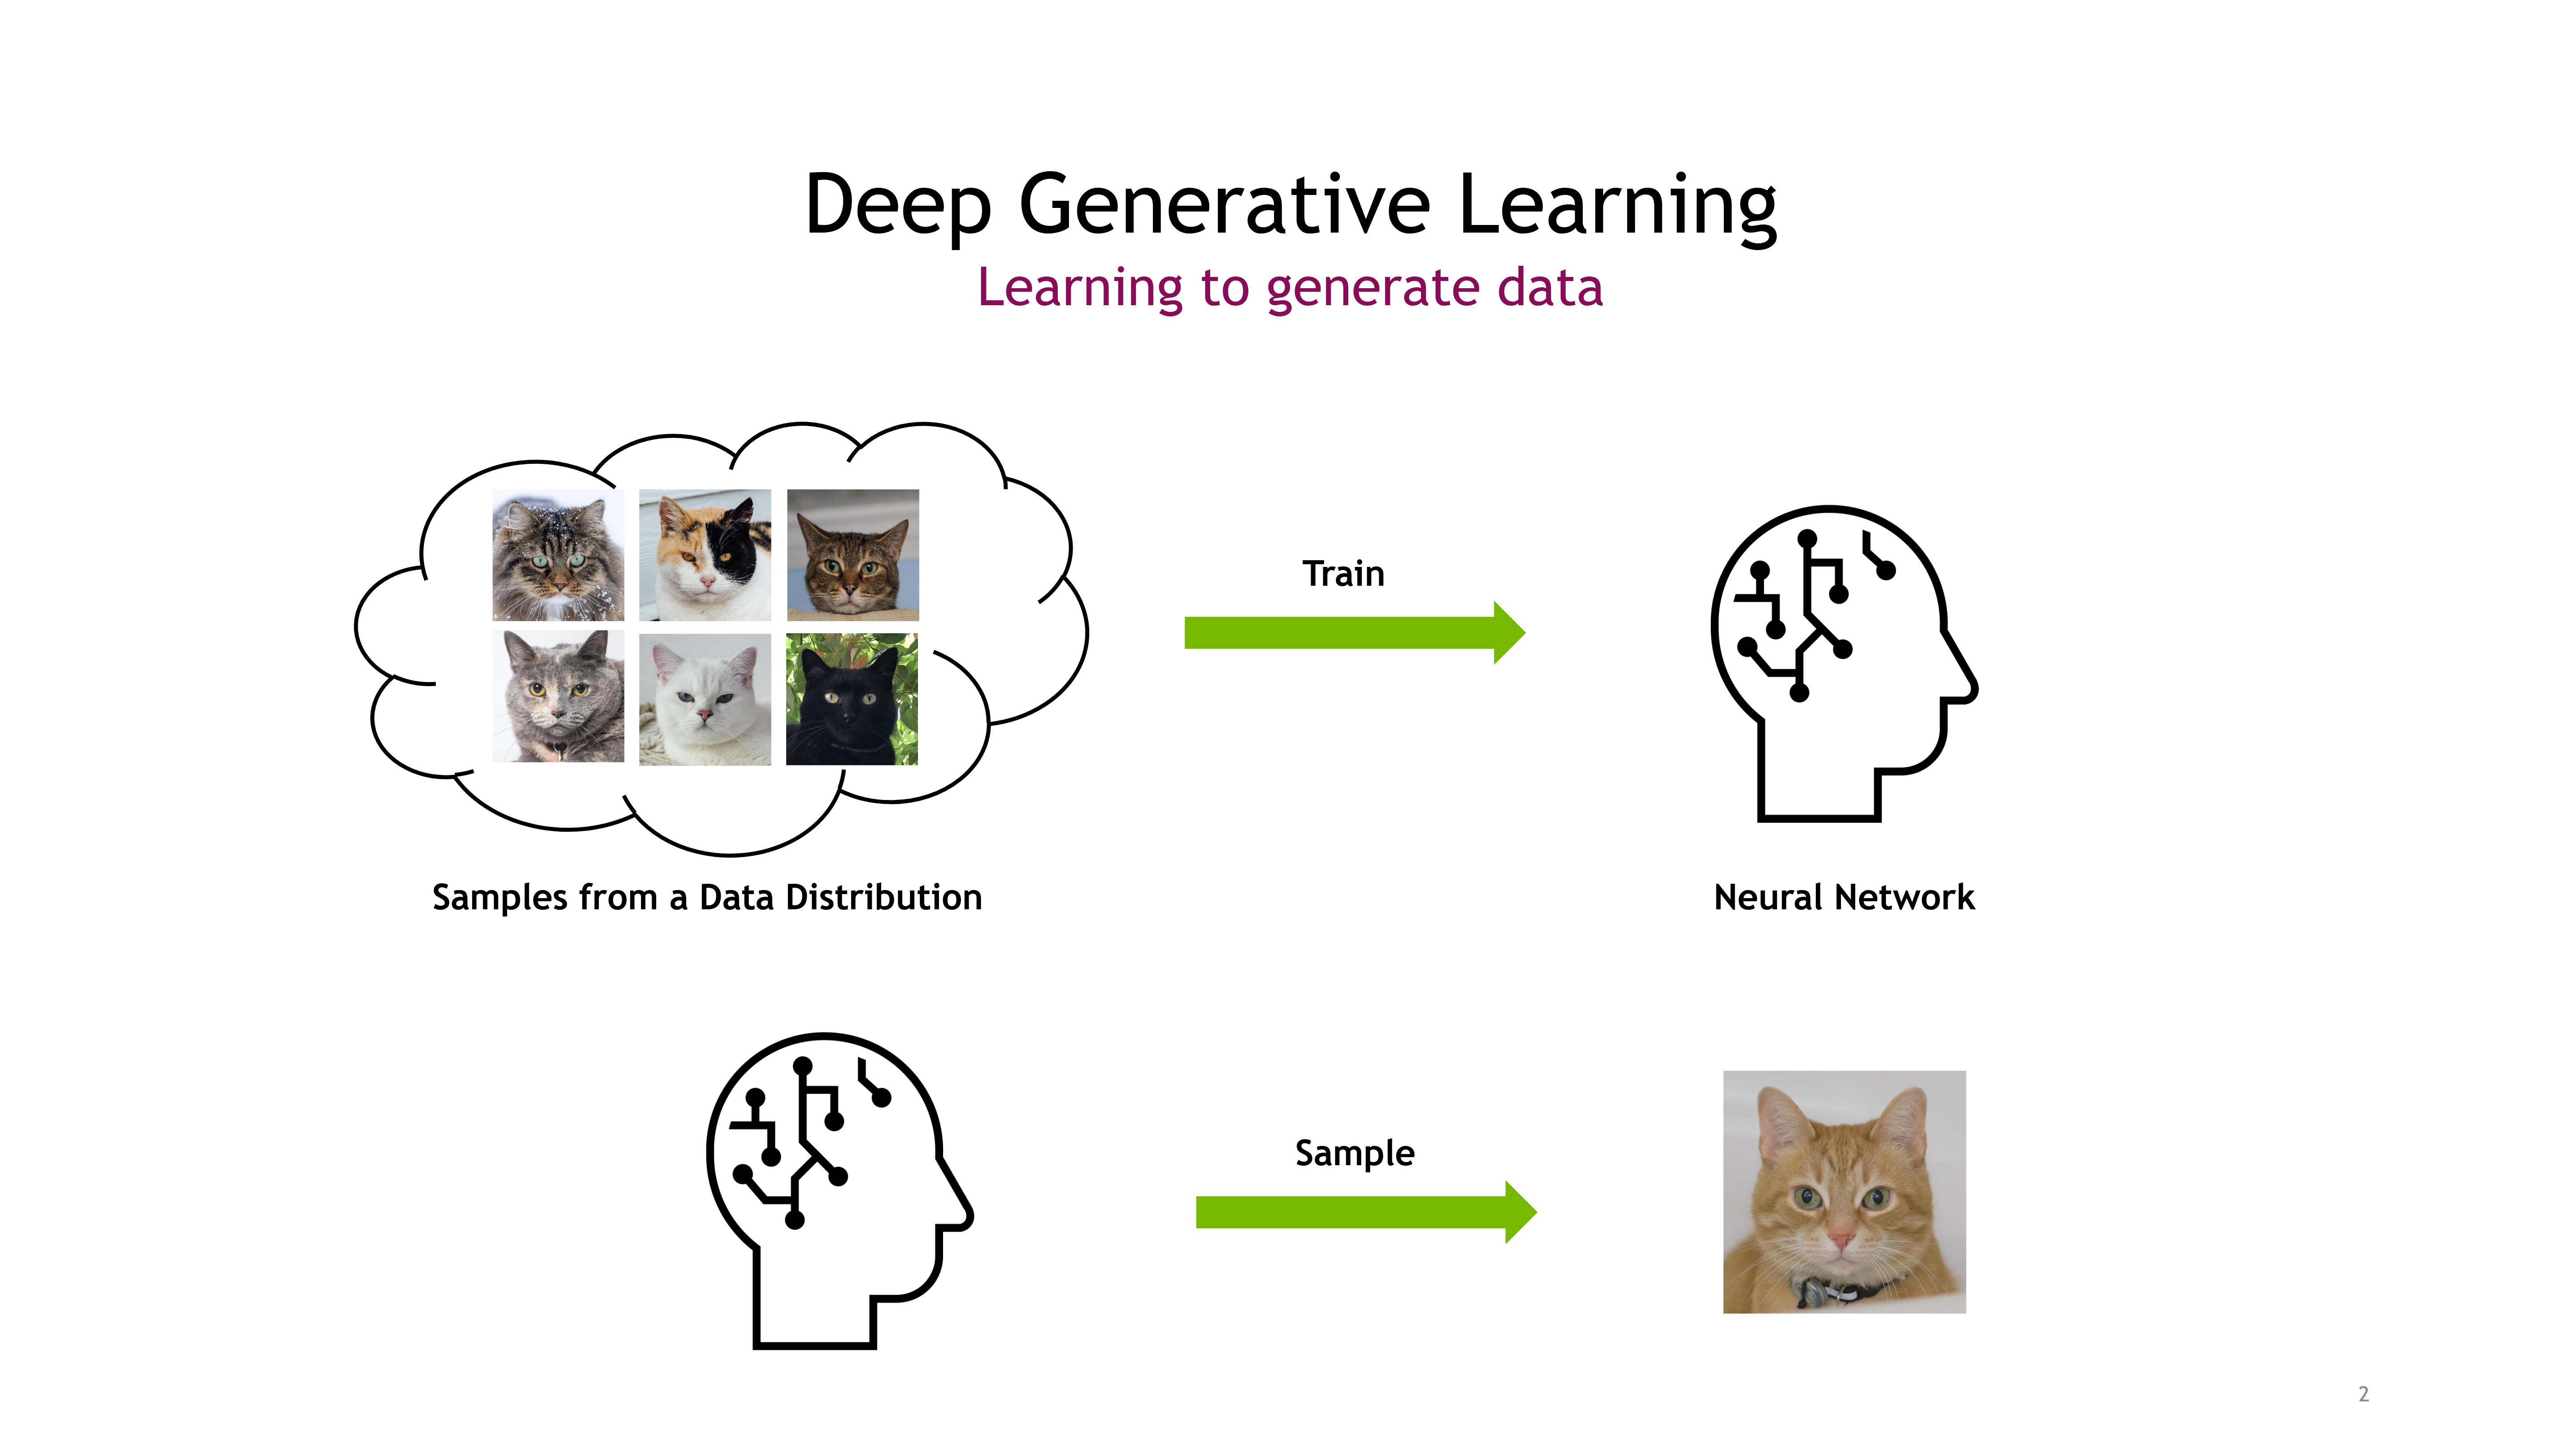
\includegraphics[width=0.8\linewidth]{learning_to_generate_data.png}
      \caption{\scriptsize Illustration of generative modeling~\parencite{CVPR2023Tutorial}.}
    \end{figure}
    
    \bottomleftrefs
  \end{frame}
\end{refsection}

\begin{refsection}
  \begin{frame}{Timeline of Generative Models}
    \begin{figure}
      \centering
      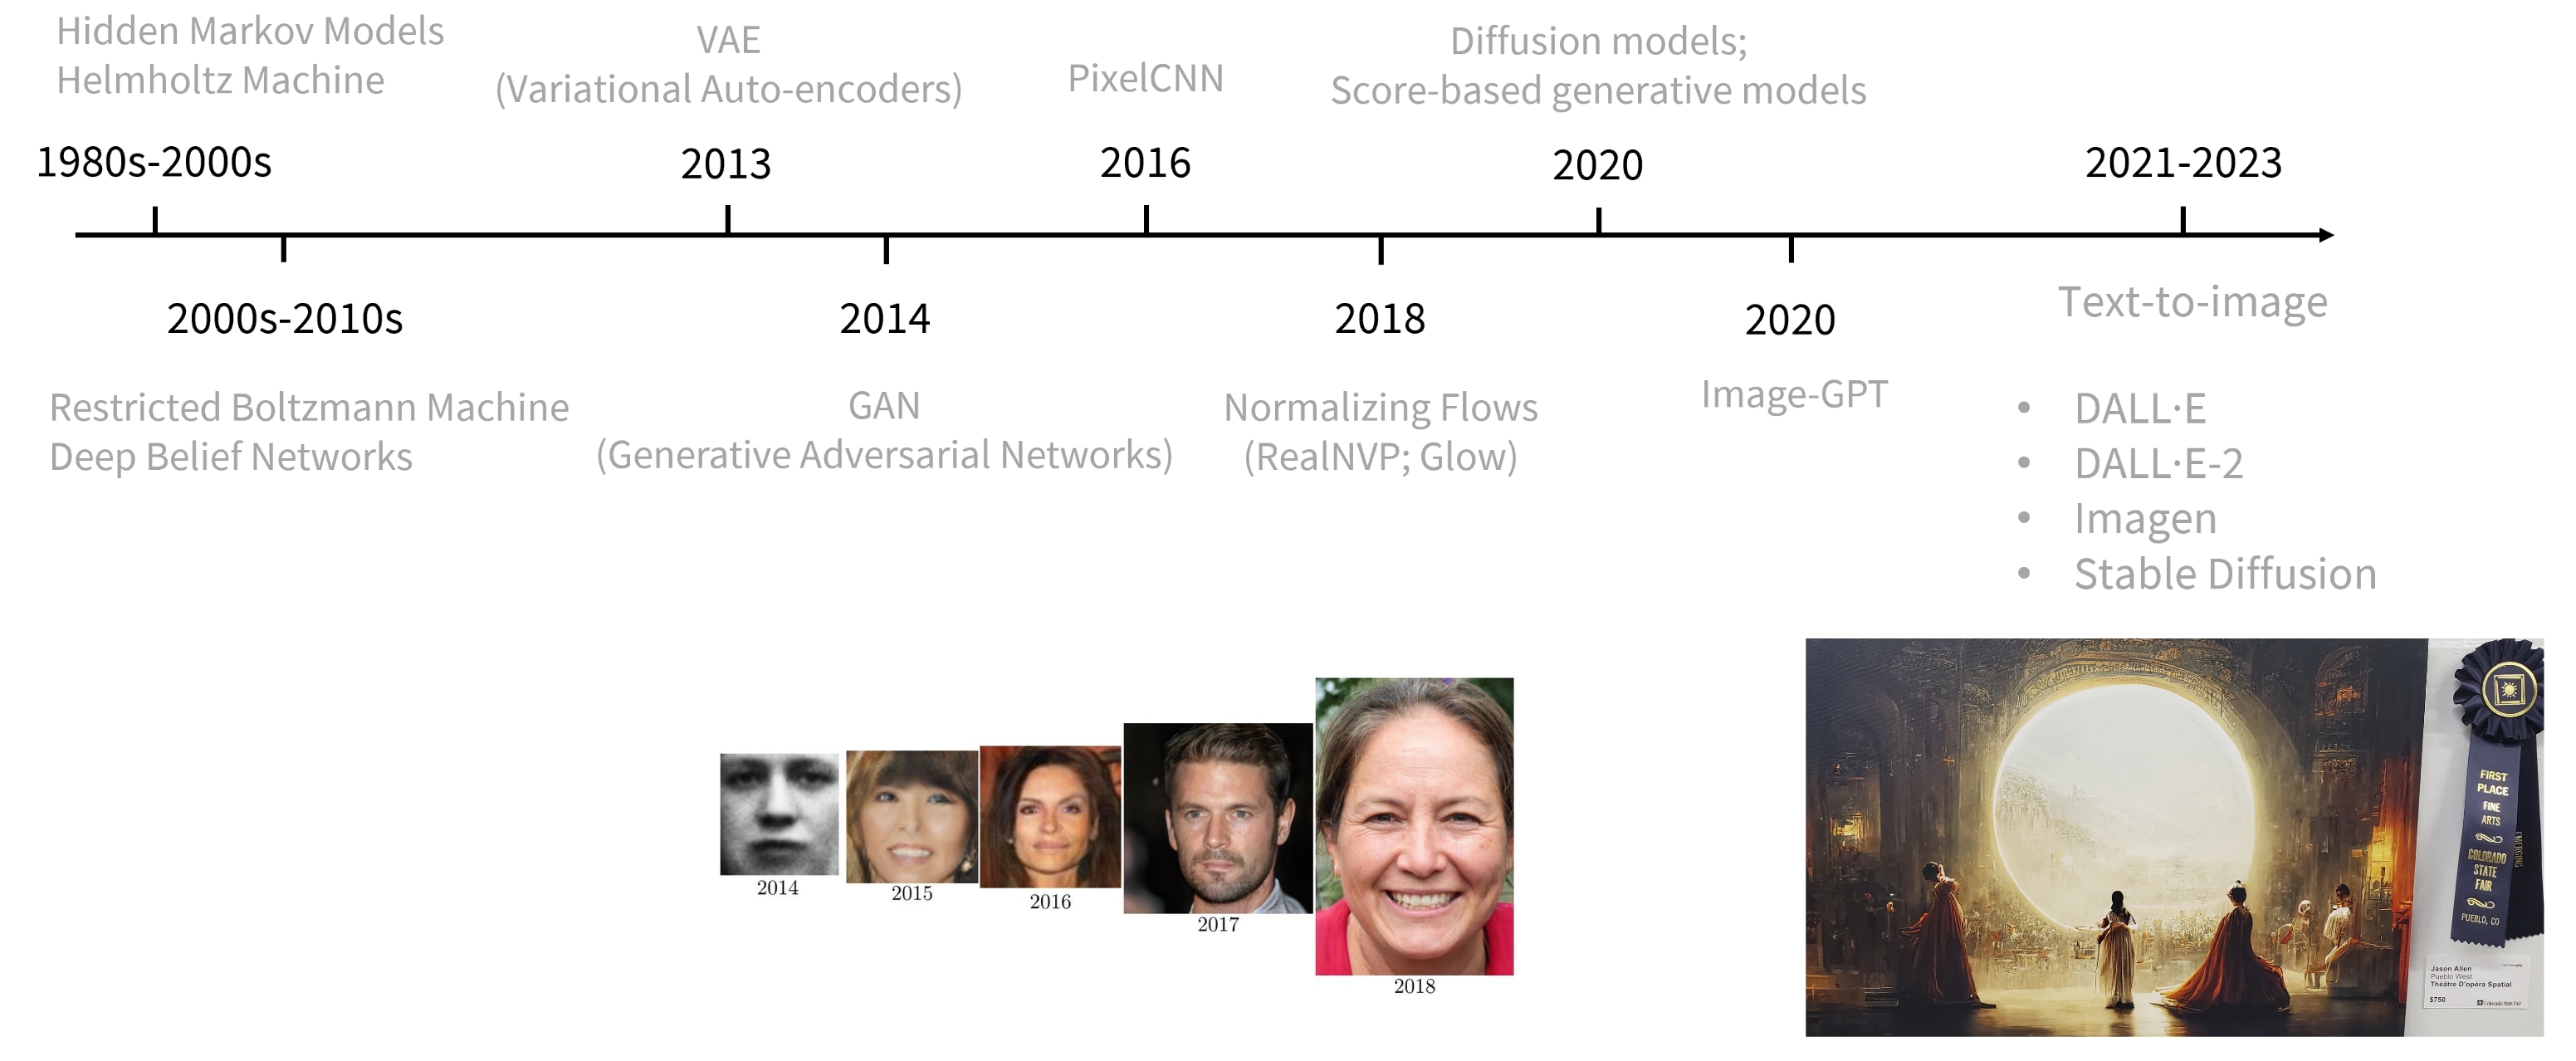
\includegraphics[width=0.95\linewidth]{genai_timeline.png}
      \caption{\scriptsize Timeline of key developments in generative models~\parencite{dengPPTAdvancedNueralNetwork2024}.}
    \end{figure}
    \bottomleftrefs
  \end{frame}
  \end{refsection}

% **2. Diffusion Models: Theory (15 min)**
%    - Intuitive explanation: what is a diffusion model?  
%    - The forward (noise) and reverse (denoise) process  
%    - How images are generated step by step  
%    - Key differences from GANs/VAEs  
%    - Strengths and weaknesses  
%    - Visual illustrations/animations

\begin{refsection}
  \begin{frame}
    \centering
    \vspace{2.5cm}
    {\LARGE \textbf{Diffusion Models: Theory}}
  \end{frame}
\end{refsection}

\begin{refsection}
  \begin{frame}{Denoising Diffusion Models}
  
    \begin{figure}
      \begin{minipage}{0.95\linewidth}
        \footnotesize
        \textbf{Denoising diffusion models consist of two processes:}
        \begin{itemize}
          \item A forward diffusion process that gradually adds noise to the input.
          \item A reverse denoising process that learns to generate data by denoising.
        \end{itemize}
      \end{minipage}
      \vspace{2em}
  
      \centering
      \includegraphics[width=1.0\linewidth]{diffusion_high_level.png}
  
      \caption[]{\scriptsize Diffusion models generate data through iterative denoising~\parencite{sohl2015deep,ho2020denoising}. \scriptsize Image credit:~\cite{CVPR2023Tutorial}.}
    \end{figure}
    \bottomleftrefs
  \end{frame}
\end{refsection}

\begin{refsection}
\begin{frame}{Forward Diffusion Process}
  \footnotesize
  The formal definition of the forward process in $T$ steps:
  \begin{center}
    \includegraphics[width=1.0\linewidth]{tutorial_diffusion_1.png}
  \end{center}
  \vspace{-1em}
    
    \begin{align*}
      q(\mathbf{x}_t \mid \mathbf{x}_{t-1}) &= \mathcal{N}\left(\mathbf{x}_t; \sqrt{1-\beta_t}\,\mathbf{x}_{t-1}, \beta_t \mathbf{I}\right)
      \hspace{1.5em}
      \Longrightarrow
      \hspace{1.5em}
      q(\mathbf{x}_{1:T} \mid \mathbf{x}_0) = \prod_{t=1}^T q(\mathbf{x}_t \mid \mathbf{x}_{t-1})
      \hspace{1.5em}
      \text{\footnotesize (joint)}
    \end{align*}
  % \vspace{1em}
  \scriptsize Image credit:~\cite{CVPR2023Tutorial}.
  \bottomleftrefs
  
\end{frame}
\end{refsection}


\begin{frame}{Forward Diffusion Process and Step-by-Step Expansion}
  \textbf{Summary of the Forward Diffusion Process:}
  \begin{align*}
      x_t = \sqrt{\alpha_t} x_{t-1} + \sqrt{1 - \alpha_t} \epsilon_t, \quad q(x_t \mid x_{t-1}) \sim \mathcal{N}\left(x_t; \sqrt{1 - \beta_t} x_{t-1}, \beta_t \mathbf{I} \right) \\
      x_t = \sqrt{\bar{\alpha}_t} x_0 + \sqrt{1 - \bar{\alpha}_t} \epsilon, \quad \bar{\alpha}_t = \prod_{i=1}^{t} \alpha_i
  \end{align*}
  \vspace{1em}
  \textbf{Detailed Step-by-Step Expansion:}
  \begin{align*}
      x_t &= \sqrt{\alpha_t} x_{t-1} + \sqrt{1 - \alpha_t} \epsilon_t \\
      x_t &= \sqrt{\alpha_t} \left( \sqrt{\alpha_{t-1}} x_{t-2} + \sqrt{1 - \alpha_{t-1}} \epsilon_{t-1} \right) + \sqrt{1 - \alpha_t} \epsilon_t \\
      x_t &= \sqrt{\alpha_t \alpha_{t-1}} x_{t-2} + \sqrt{\alpha_t} \sqrt{1 - \alpha_{t-1}} \epsilon_{t-1} + \sqrt{1 - \alpha_t} \epsilon_t \\
      x_t &= \sqrt{\alpha_t \alpha_{t-1} \alpha_{t-2}} x_{t-3} + \cdots + \sqrt{1 - \alpha_t \alpha_{t-1}} \epsilon \\
      x_t &= \sqrt{\bar{\alpha}_t} x_0 + \sqrt{1 - \bar{\alpha}_t} \epsilon \\
      % \bar{\alpha}_t &= \prod_{i=1}^{t} \alpha_i
  \end{align*}
\end{frame}


\begin{refsection}
\begin{frame}{Diffusion Kernel}
  \begin{figure}
    \centering
    \includegraphics[width=1.0\linewidth]{diffusion_kernel.png}
  \end{figure}

  \vspace{-2em}

  {\small
  \begin{flushleft}
  \begin{align*}
    &\textbf{Define:} \qquad \overline{\alpha}_t = \prod_{s=1}^t (1 - \beta_s)
    &\implies q(\mathbf{x}_t \mid \mathbf{x}_0) = \mathcal{N}\left(\mathbf{x}_t; \sqrt{\overline{\alpha}_t}\, \mathbf{x}_0, (1 - \overline{\alpha}_t)\mathbf{I}\right) \hspace{1em} \text{\footnotesize (Diffusion Kernel)}
  \end{align*}
  \end{flushleft}
  }
  \vspace{-1em}
  {\small
  \begin{flushleft}
  \begin{align*}
    &\textbf{For sampling:} \qquad \mathbf{x}_t = \sqrt{\overline{\alpha}_t}\, \mathbf{x}_0 + \sqrt{1 - \overline{\alpha}_t}\, \boldsymbol{\epsilon}
    &\text{where} \quad \boldsymbol{\epsilon} \sim \mathcal{N}(\mathbf{0}, \mathbf{I})
  \end{align*}
  \end{flushleft}
  }

  \begin{flushleft}
  \footnotesize
  The noise schedule $\{\beta_t\}$ is chosen so that $\overline{\alpha}_T \to 0$ and $q(\mathbf{x}_T \mid \mathbf{x}_0) \approx \mathcal{N}(\mathbf{x}_T; \mathbf{0}, \mathbf{I})$.
  \end{flushleft}

  \scriptsize Image credit:~\cite{CVPR2023Tutorial}.
  \bottomleftrefs
\end{frame}
\end{refsection}

\begin{refsection}
  \begin{frame}{What happens to a distribution in the forward diffusion?}
      So far, we discussed the diffusion kernel $q(\mathbf{x}_t|\mathbf{x}_0)$ but what about $q(\mathbf{x}_t)$?

      \vspace{1em}

        \centering
        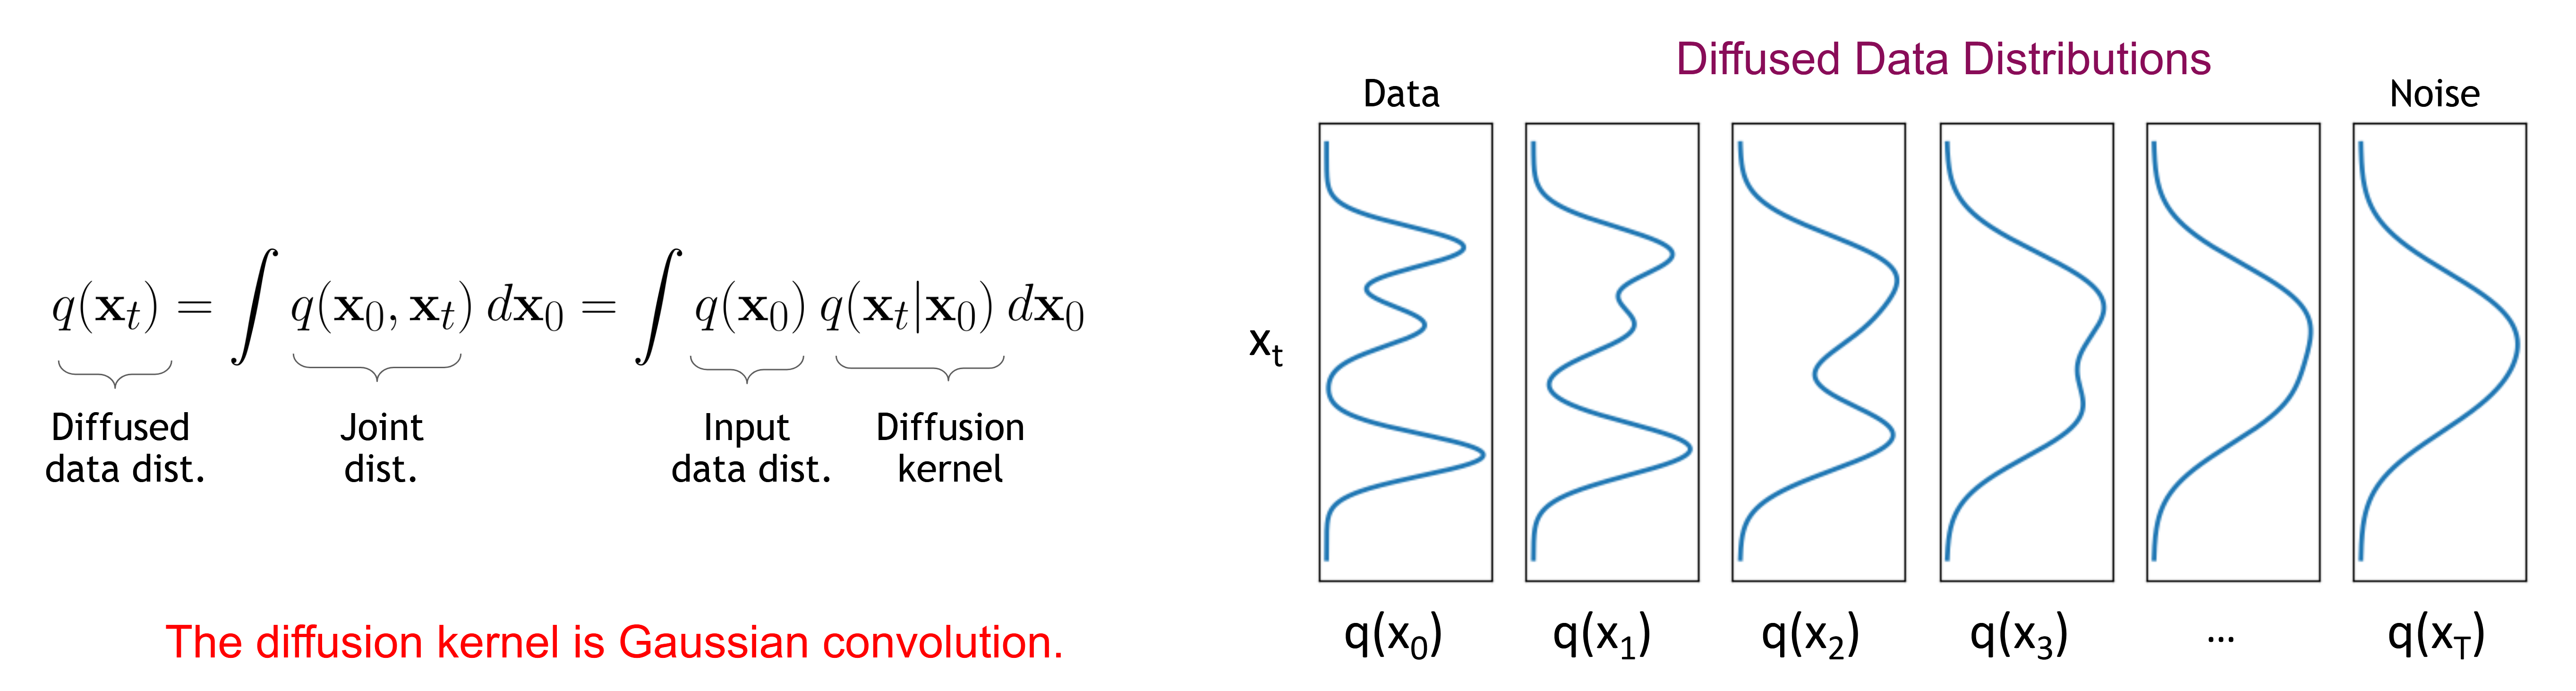
\includegraphics[width=\linewidth]{diffused_data_distributions.png}
  % \vspace{1em}

  
      We can sample $\mathbf{x}_t \sim q(\mathbf{x}_t)$ by first sampling $\mathbf{x}_0 \sim q(\mathbf{x}_0)$ and then sampling $\mathbf{x}_t \sim q(\mathbf{x}_t|\mathbf{x}_0)$ (i.e., ancestral sampling).
     
      \scriptsize Image credit:~\cite{CVPR2023Tutorial}.
      \bottomleftrefs
  \end{frame}
  \end{refsection}


\begin{refsection}
\begin{frame}{Generative Learning by Denoising}
  Recall that the diffusion parameters are designed such that $q(\mathbf{x}_T) \approx \mathcal{N}(\mathbf{x}_T; 0, \mathbf{I})$.
  \begin{columns}
    \begin{column}{0.4\textwidth}
      \textbf{Generation:}
      \begin{itemize}
        \item Sample $\mathbf{x}_T \sim \mathcal{N}(\mathbf{x}_T; 0, \mathbf{I})$
        \item Iteratively sample $\mathbf{x}_{t-1} \sim \underbrace{q(\mathbf{x}_{t-1} \mid \mathbf{x}_t)}_{\text{True Denoising Dist.}}$
      \end{itemize}
    \end{column}
    \begin{column}{0.6\textwidth}
      \centering
      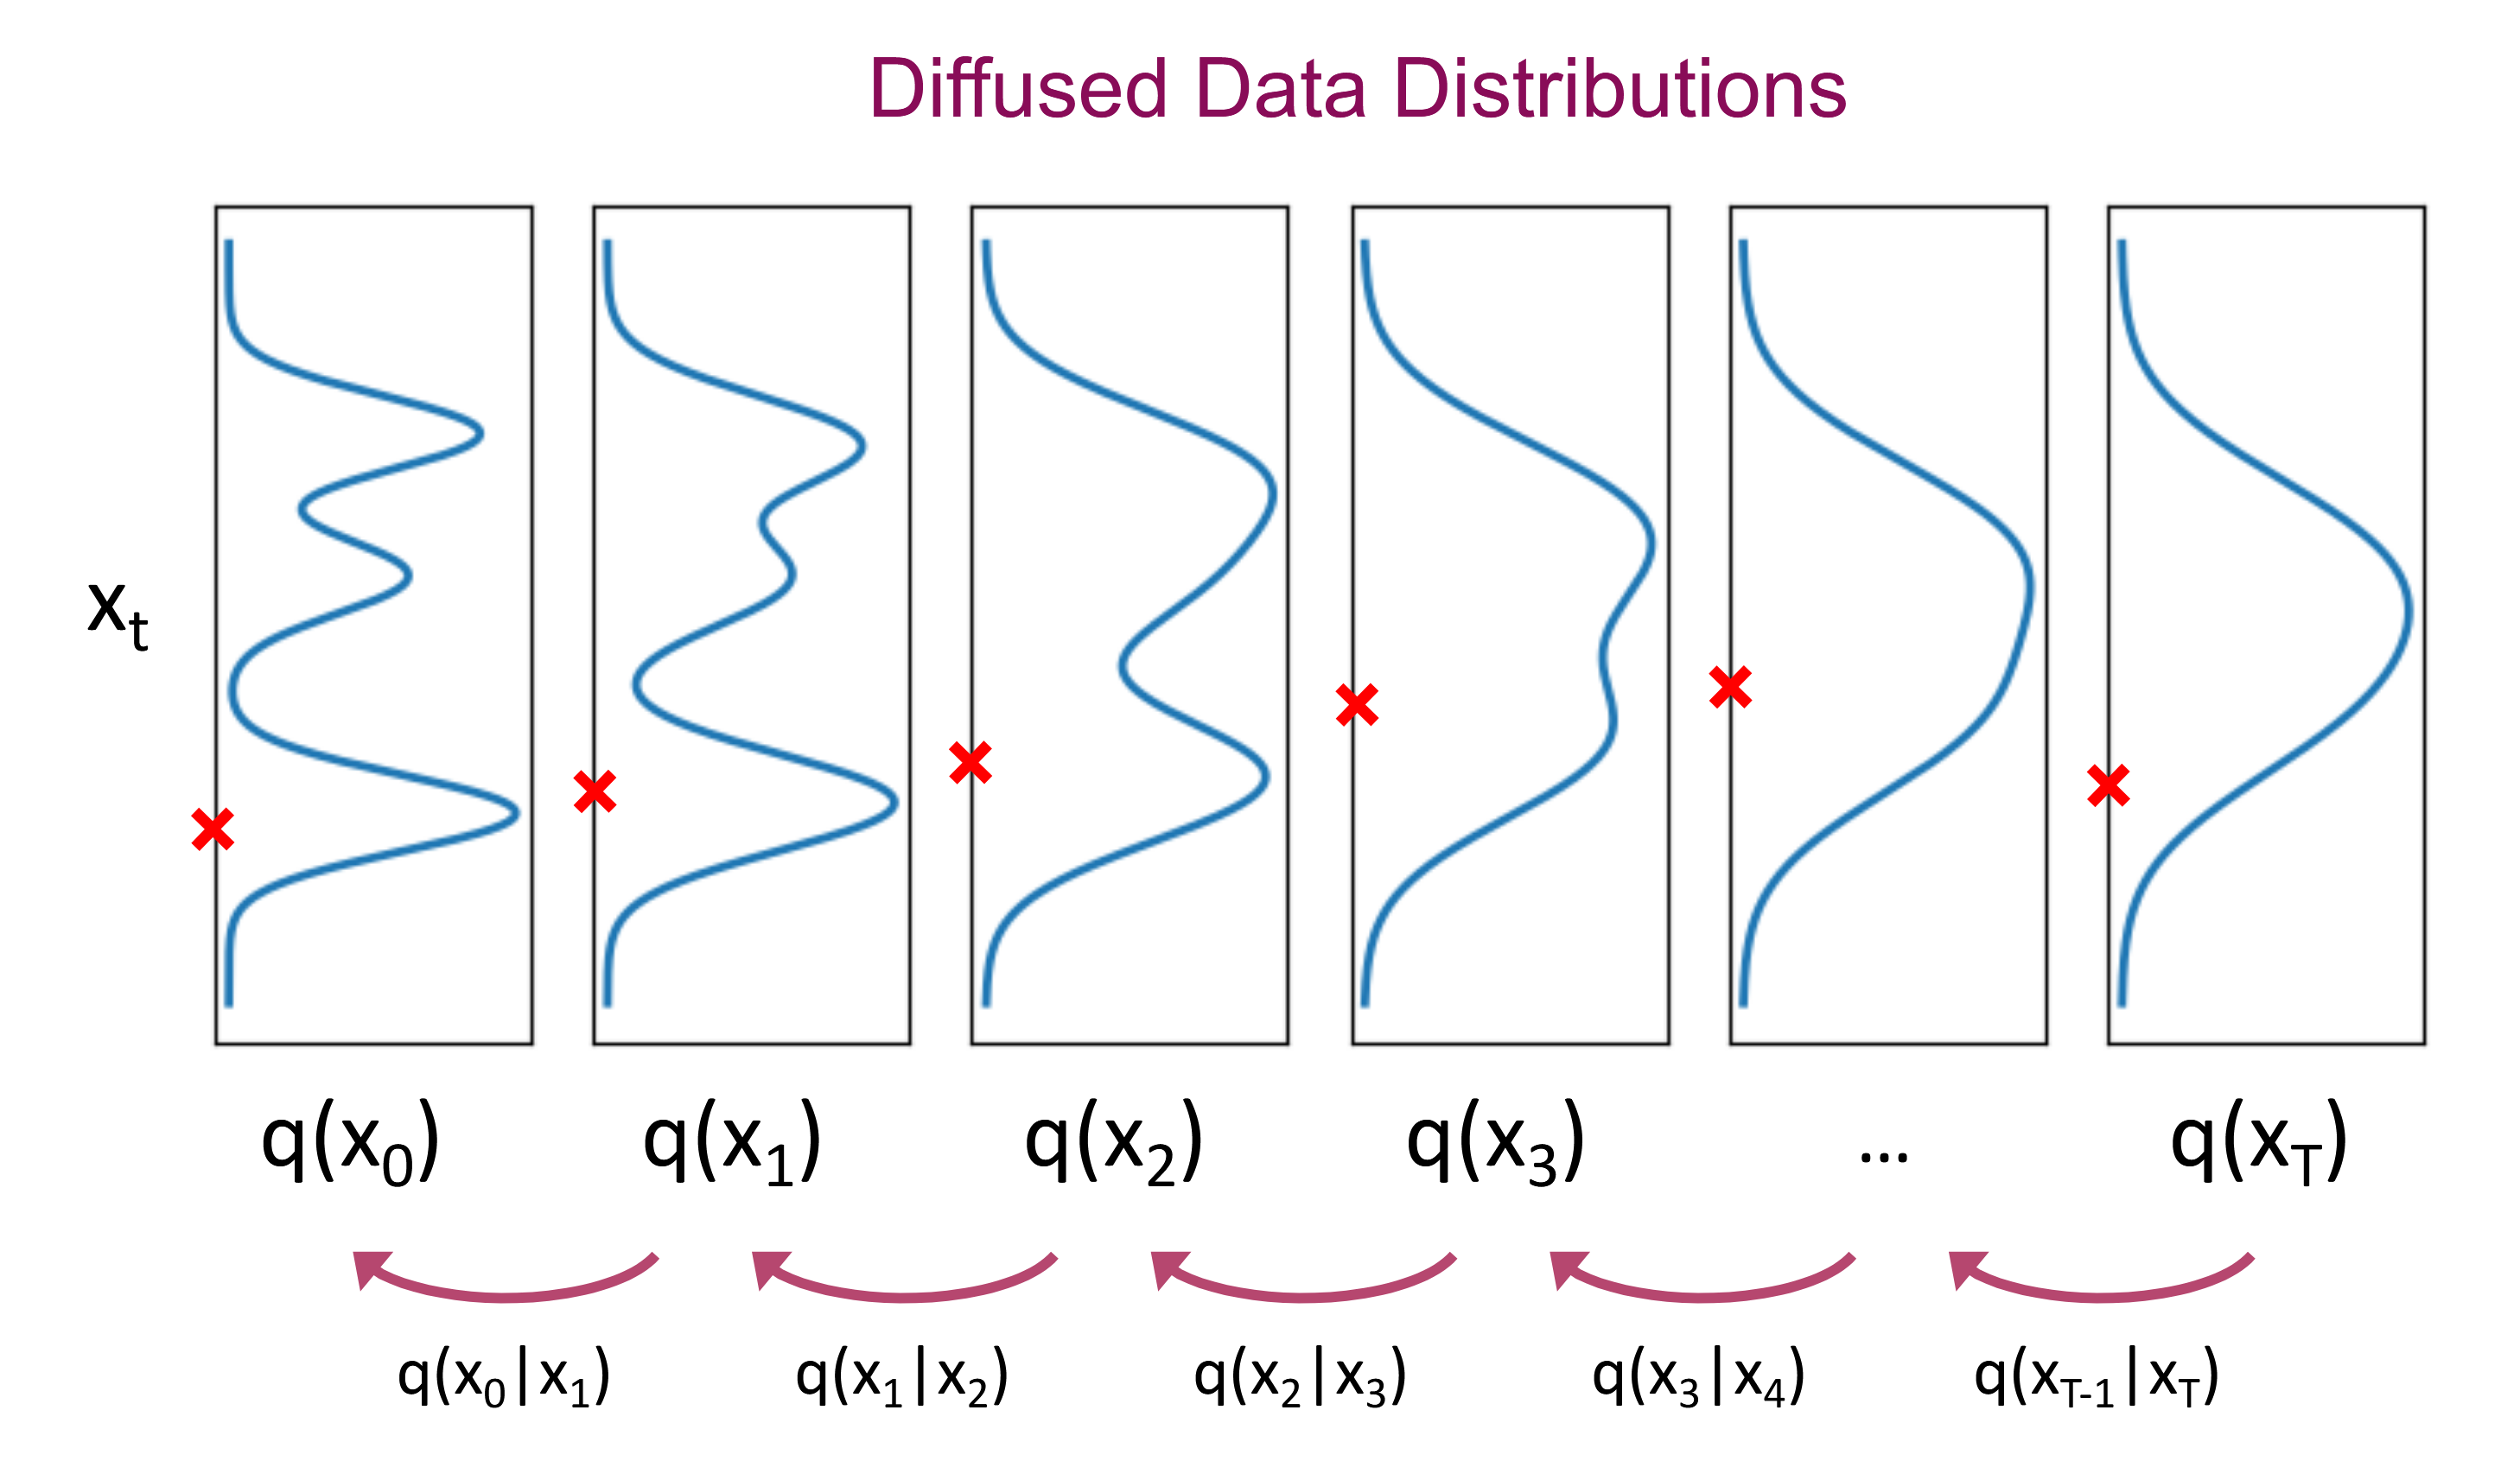
\includegraphics[width=1.0\linewidth]{generative_learning_by_denoising.png}
    \end{column}
  \end{columns}
  Can we approximate $q(\mathbf{x}_{t-1} \mid \mathbf{x}_t)$? Yes, we can use a \textcolor{green}{normal distribution} if $\beta_t$ is small in each forward diffusion step.

  \scriptsize Image credit:~\cite{CVPR2023Tutorial}.
  \bottomleftrefs
\end{frame}
\end{refsection}

\begin{refsection}
\begin{frame}{Reverse Denoising Process}
  Formal definition of forward and reverse processes in $T$ steps:
  \begin{center}
    \includegraphics[width=1.0\linewidth]{reverse_denoising_process.png}
  \end{center}
  \vspace{-2em}
  \begin{align*}
    p(x_T) &= \mathcal{N}(x_T; 0, I) \\
    p_\theta(x_{t-1}\mid x_t)
    &= \mathcal{N}\bigl(x_{t-1};\,\mu_\theta(x_t, t),\,\sigma_t^2 I\bigr)\quad
    \Rightarrow\quad
    p_\theta(x_{0:T})
    &= p(x_T)\,\prod_{t=1}^T p_\theta(x_{t-1}\mid x_t).
  \end{align*}
    \scriptsize
    where $\mu_\theta(x_t, t)$ is a trainable network (e.g., U-Net, Denoising Autoencoder)

    \scriptsize Image credit:~\cite{CVPR2023Tutorial}.
    \bottomleftrefs
\end{frame}
\end{refsection}

\begin{refsection}
\begin{frame}{Learning Denoising Model}
  \begin{minipage}{1.0\linewidth}
  \centering
  {\color{purple}\scriptsize Variational upper bound}
  \vspace{0.3em}

  \begin{itemize}
    \setlength\itemsep{0.2em}
    \item {\scriptsize For training, use a variational upper bound (as in VAEs):}
    {\scriptsize
    \begin{align*}
      \mathbb{E}_{q_\lambda} [ \log p_\theta(\mathbf{x}) ] \leq \mathbb{E}_{q_\lambda} \left[ \log \frac{p_\theta(\mathbf{x}, \mathbf{z})}{q_\lambda(\mathbf{z}|\mathbf{x})} \right] = L
    \end{align*}
    }
    \item {\scriptsize $\mathbf{x}_t = \sqrt{\bar{\alpha}_t} \mathbf{x}_0 + \sqrt{1 - \bar{\alpha}_t} \boldsymbol{\epsilon}$, mean parameterized as~\parencite{ho2020denoising}:}
    {\scriptsize
    \begin{align*}
      \mu_\theta(\mathbf{x}_t, t) = \frac{1}{\sqrt{\alpha_t}} \left( \mathbf{x}_t - \frac{1 - \alpha_t}{\sqrt{1 - \bar{\alpha}_t}} \boldsymbol{\epsilon}_\theta(\mathbf{x}_t, t) \right)
    \end{align*}
    }
    \item {\scriptsize Variational objective:}
    {\scriptsize
    \begin{align*}
      L = \mathbb{E}_{q(\mathbf{x}_0, \boldsymbol{\epsilon})} \left[ \sum_{t=1}^T \lambda_t \mathbb{E}_{q(\mathbf{x}_t|\mathbf{x}_0)} \left[ \left\| \boldsymbol{\epsilon} - \boldsymbol{\epsilon}_\theta(\sqrt{\bar{\alpha}_t} \mathbf{x}_0 + \sqrt{1 - \bar{\alpha}_t} \boldsymbol{\epsilon}, t) \right\|^2 \right] \right]
    \end{align*}
    }
    \item {\scriptsize Set $\lambda_t=1$ for all $t$ works best~\parencite{ho2020denoising}.}
  \end{itemize}
  \end{minipage}
  \vspace{-0.5em}
  \bottomleftrefs
\end{frame}
\end{refsection}

\begin{refsection}
\begin{frame}{Summary}
  \centering
  {\color{purple} \small Training and Sample Generation}
  \vspace{1em}

  \begin{minipage}{0.45\linewidth}
    \scriptsize
    \textbf{Algorithm1-Training}
    \vspace{0.5em}
    \renewcommand{\arraystretch}{1.5}
    \begin{tabular}{l}
      \toprule
      1: \quad \textbf{repeat} \\
      2: \quad \hspace{1em} $\mathbf{x}_0 \sim q(\mathbf{x}_0)$ \\
      3: \quad \hspace{1em} $t \sim \mathrm{Uniform}(\{1, \ldots, T\})$ \\
      4: \quad \hspace{1em} $\boldsymbol{\epsilon} \sim \mathcal{N}(0, I)$ \\
      5: \quad \hspace{1em} Take gradient descent step on \\
      \quad \hspace{2.5em} $\nabla_\theta \left\| \boldsymbol{\epsilon} - \boldsymbol{\epsilon}_\theta\left(\sqrt{\bar{\alpha}_t} \mathbf{x}_0 + \sqrt{1 - \bar{\alpha}_t} \boldsymbol{\epsilon}, t\right) \right\|^2$ \\
      6: \quad \textbf{until converged} \\
      \bottomrule
    \end{tabular}
  \end{minipage}
  \hfill
  \renewcommand{\arraystretch}{1.5}
  \begin{minipage}{0.45\linewidth}
    \scriptsize
    \textbf{Algorithm2-Sampling}
    \vspace{0.5em}
    \begin{tabular}{l}
      \toprule
      1: \quad $\mathbf{x}_T \sim \mathcal{N}(0, I)$ \\
      2: \quad \textbf{for} $t = T, \ldots, 1$ \textbf{do} \\
      3: \quad \hspace{1em} $\mathbf{z} \sim \mathcal{N}(0, I)$ \\
      4: \quad \hspace{1em} $\mathbf{x}_{t-1} = \frac{1}{\sqrt{\alpha_t}} \left( \mathbf{x}_t - \frac{1 - \alpha_t}{\sqrt{1 - \bar{\alpha}_t}} \boldsymbol{\epsilon}_\theta(\mathbf{x}_t, t) \right) + \sigma_t \mathbf{z}$ \\
      5: \quad \textbf{end for} \\
      6: \quad \textbf{return} $\mathbf{x}_0$ \\
      \bottomrule
    \end{tabular}
  \end{minipage}
  \renewcommand{\arraystretch}{1}
  \vspace{1em}
  Algorithms are derived from~\parencite{ho2020denoising}
  \bottomleftrefs
\end{frame}
\end{refsection}


% **3. Applications in Remote Sensing (12 min)**
%    - Data augmentation for training  
%    - Super-resolution of satellite images  
%    - Cloud removal and inpainting  
%    - Synthetic data for rare events  
%    - Real-world case studies and visual results



\begin{refsection}
  \begin{frame}
    \centering
    \vspace{2.5cm}
    {\LARGE \textbf{Applications in Remote Sensing}}
  \end{frame}
\end{refsection}


\begin{refsection}
  \begin{frame}{Introduction to DiffusionSat}
    \begin{figure}
      \centering
      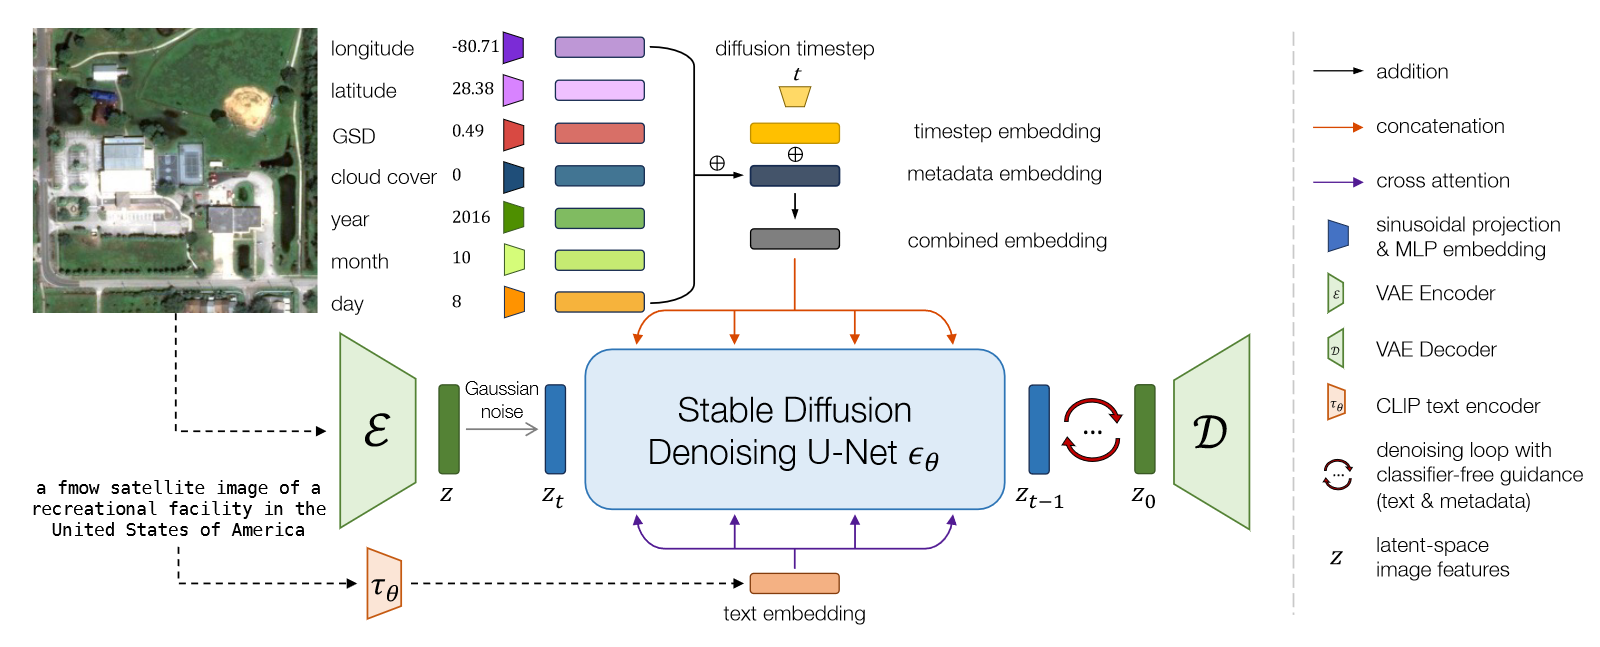
\includegraphics[width=0.85\linewidth]{diffusionsat_base.png}
      \caption{\scriptsize Overall architecture of the DiffusionSat \emph{base} model, showing how freely-available metadata (sensor type, date, location) is fused with a diffusion backbone to generate high-fidelity satellite imagery~\parencite{diffusionset2024}.}
    \end{figure}
    \bottomleftrefs
  \end{frame}
\end{refsection}

\begin{refsection}
  \begin{frame}{Text Encoder in DiffusionSat}
    \begin{columns}[t]
      \begin{column}{0.4\textwidth}
        \small
        \begin{itemize}
          \item \textbf{Input Prompt:} \texttt{"A satellite image of a farmland"}
          \item \textbf{Tokenization:}
          \begin{itemize}
            \item Split into subwords $\rightarrow$ tokens
            \item Example mapping: \(\{\text{"A"}:101,\ \text{" satellite"}:564,\ \dots,\ \texttt{<EOS>}:102\}\)
          \end{itemize}
          \item \textbf{CLIP Text Encoder:}
          \begin{itemize}
            \item Token IDs $\rightarrow$ 512-dim embedding
            \item Captures semantic features
          \end{itemize}
        \end{itemize}
      \end{column}
      \begin{column}{0.6\textwidth}
        \begin{figure}
          \centering
          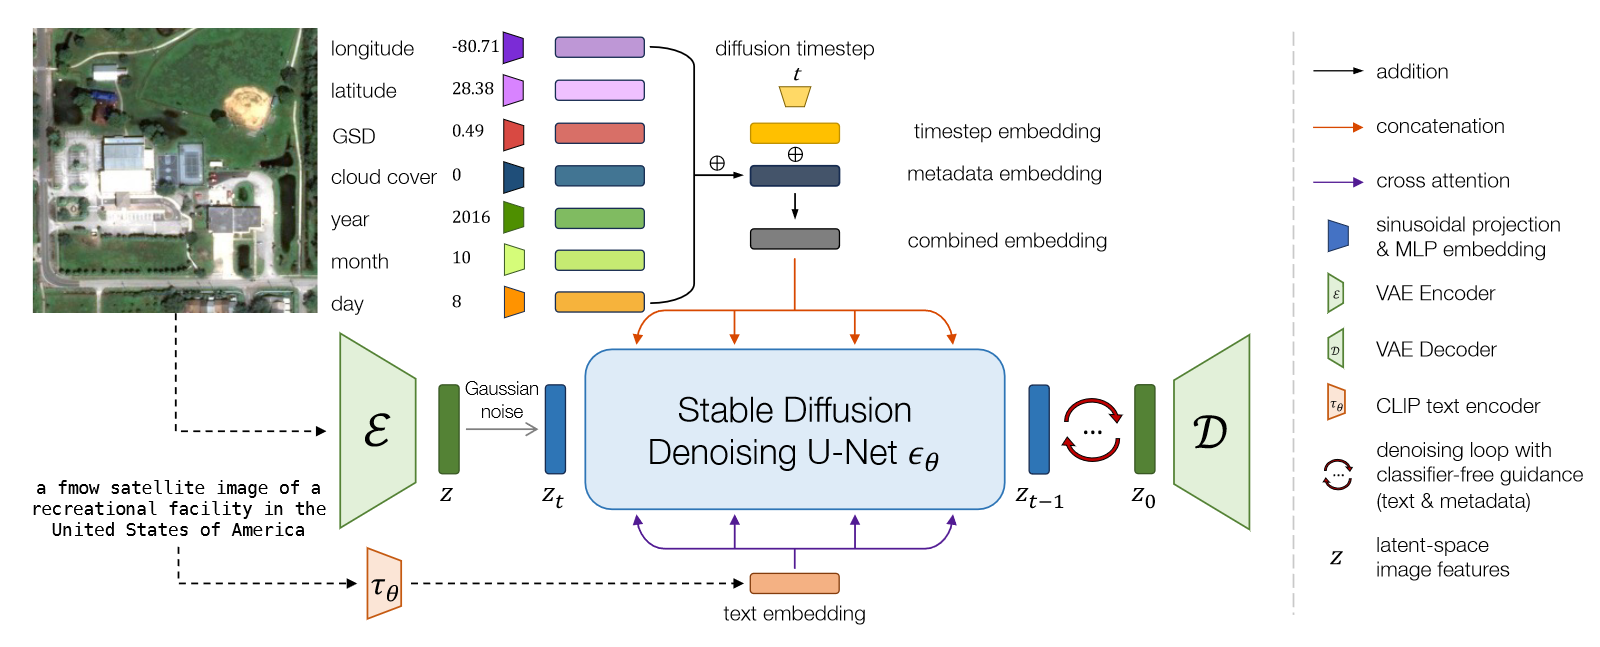
\includegraphics[width=\linewidth]{diffusionsat_base.png}
          \caption{\scriptsize The text encoder module (OpenAI CLIP) tokenizes the input prompt and produces a 512-dimensional embedding to condition the diffusion backbone~\parencite{diffusionset2024}.}
        \end{figure}
      \end{column}
    \end{columns}
    \bottomleftrefs
  \end{frame}
\end{refsection}

\begin{refsection}
  \begin{frame}{Metadata Encoder in DiffusionSat}
    \begin{columns}[t]
      \begin{column}{0.4\textwidth}
        \small
        \begin{itemize}
          \item \textbf{Input Metadata Example:}
          \begin{itemize}
            \item Sensor: Sentinel-2
            \item Location: (lat: 37.7749, lon: -122.4194)
            \item Date: 2022-06-01
            \item GSD: 10 m
            \item Cloud cover: 5\%
          \end{itemize}
          \item \textbf{Processing Module:} Metadata Encoder
          \item \textbf{Output:} 512-dim conditioning embedding
        \end{itemize}
      \end{column}
      \begin{column}{0.6\textwidth}
        \begin{figure}
          \centering
          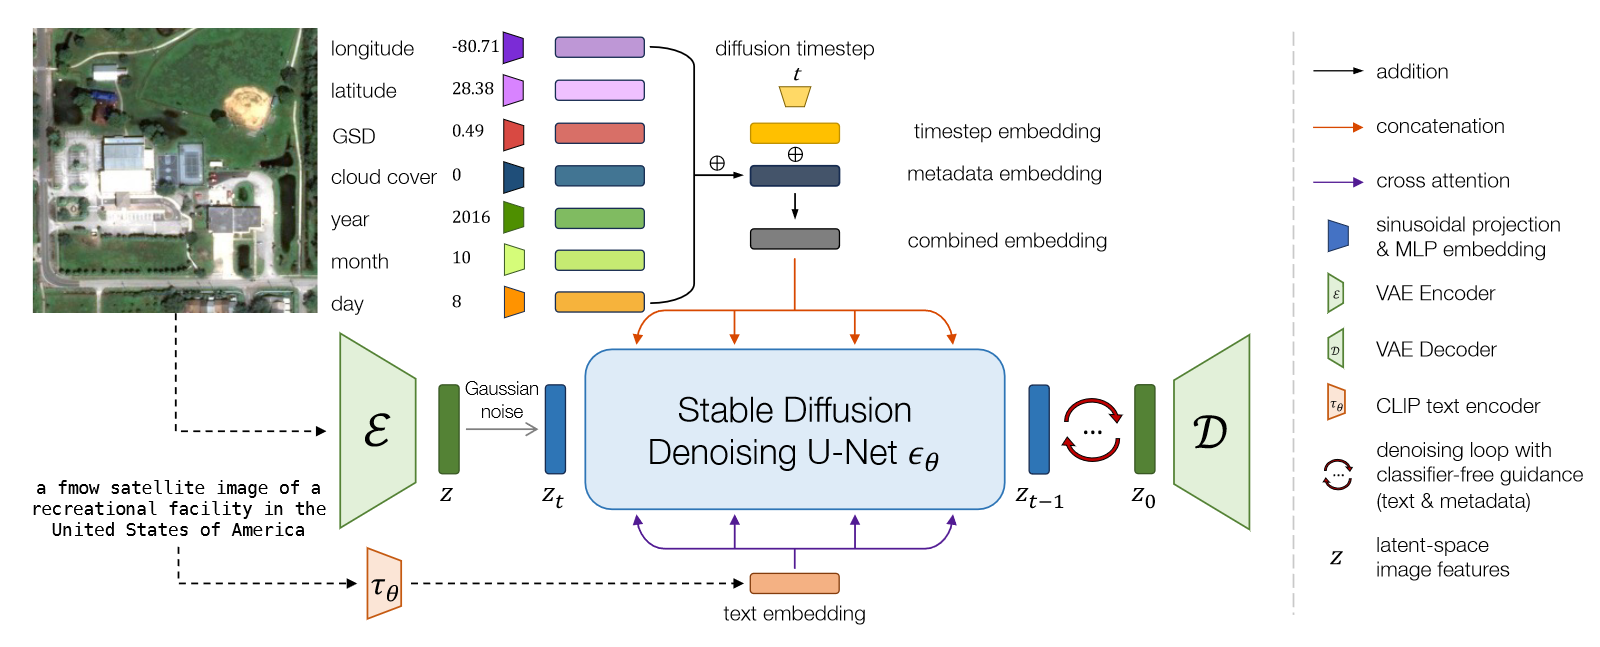
\includegraphics[width=\linewidth]{diffusionsat_base.png}
          \caption{\scriptsize The Metadata Encoder transforms raw satellite metadata into a fixed-length embedding to condition the diffusion backbone~\parencite{diffusionset2024}.}
        \end{figure}
      \end{column}
    \end{columns}
    \bottomleftrefs
  \end{frame}
\end{refsection}

\begin{refsection}
  \begin{frame}{Image Processing \& Diffusion Steps}
    \begin{columns}[t]
      \begin{column}{0.5\textwidth}
        \tiny
        \begin{itemize}
          \item \textbf{Training Process:}
          \begin{itemize}
            \item Input: Clean satellite image
            \item Encode: Image Encoder $\rightarrow$ latent
            \item Forward Diffusion: Add Gaussian noise over \(T\) steps
            \item Conditioning: Inject Text \& Metadata embeddings
            \item Learn: UNet predicts and removes noise
          \end{itemize}
          \item \textbf{Inference Process:}
          \begin{itemize}
            \item Input: Random noise latent \(x_T\!\sim\!\mathcal{N}(0,I)\)
            \item Reverse Diffusion: Iteratively denoise via UNet (conditioned)
            \item Decode: Latent Decoder $\rightarrow$ final high-fidelity image
          \end{itemize}
        \end{itemize}
      \end{column}
      \begin{column}{0.5\textwidth}
        \begin{figure}
          \centering
          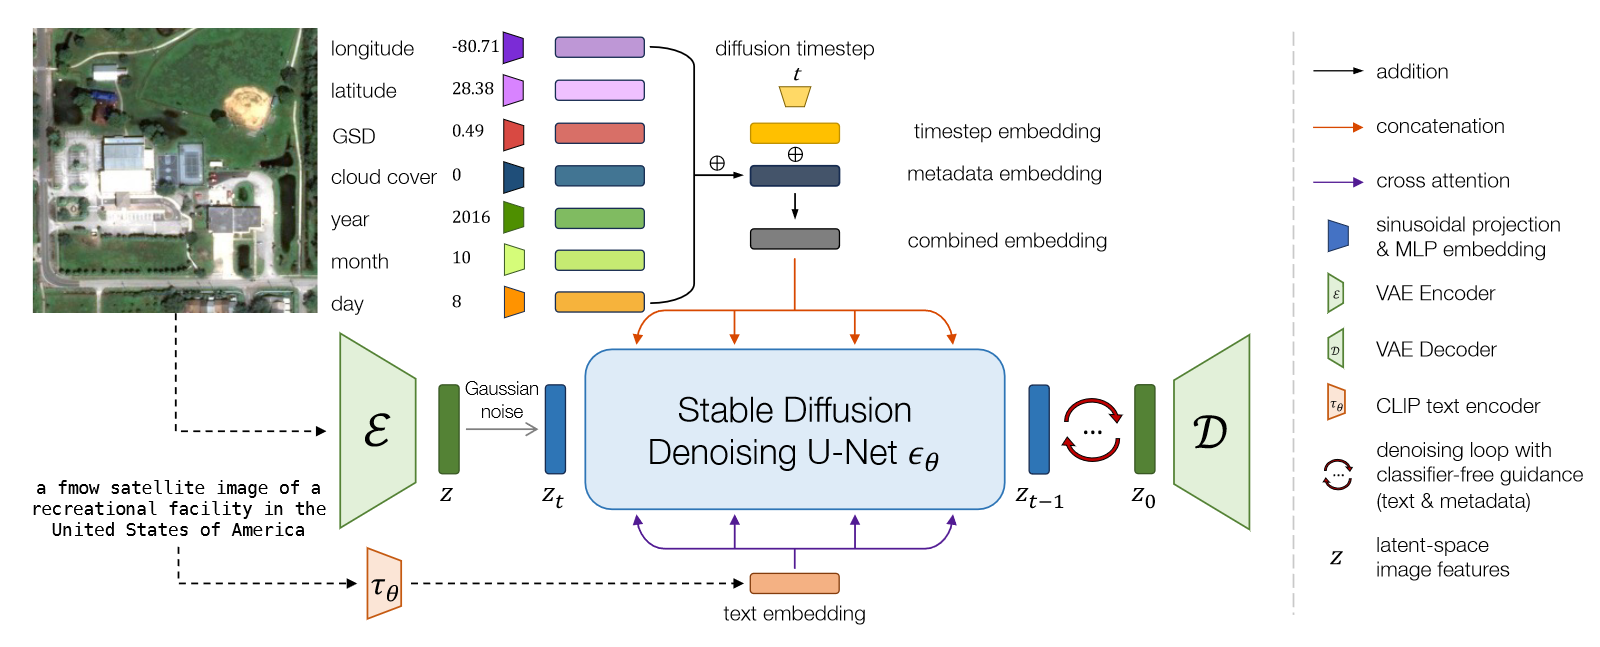
\includegraphics[width=\linewidth]{diffusionsat_base.png}
          \caption{\scriptsize Comparison of the training (forward diffusion) and inference (reverse denoising) pipelines in the DiffusionSat base model, showing how images traverse the encoders, diffusion backbone, and decoder~\parencite{diffusionset2024}.}
        \end{figure}
      \end{column}
    \end{columns}
    \bottomleftrefs
  \end{frame}
\end{refsection}

\begin{refsection}
  \begin{frame}{Reverse Diffusion: Sampling}
    \begin{columns}[t]
      \begin{column}{0.4\textwidth}
        \small
        \begin{itemize}
          \item \textbf{High-Level Sampling:} \(x \sim p(\text{noise},\,c_{\text{text}},\,c_{\text{meta}})\)
          \item \textbf{Where:}
          \begin{itemize}
            \item noise: \(x_T\!\sim\!\mathcal{N}(0,I)\)
            \item \(c_{\text{text}}\): text embedding
            \item \(c_{\text{meta}}\): metadata embedding
          \end{itemize}
        \end{itemize}
      \end{column}
      \begin{column}{0.6\textwidth}
        \begin{figure}
          \centering
          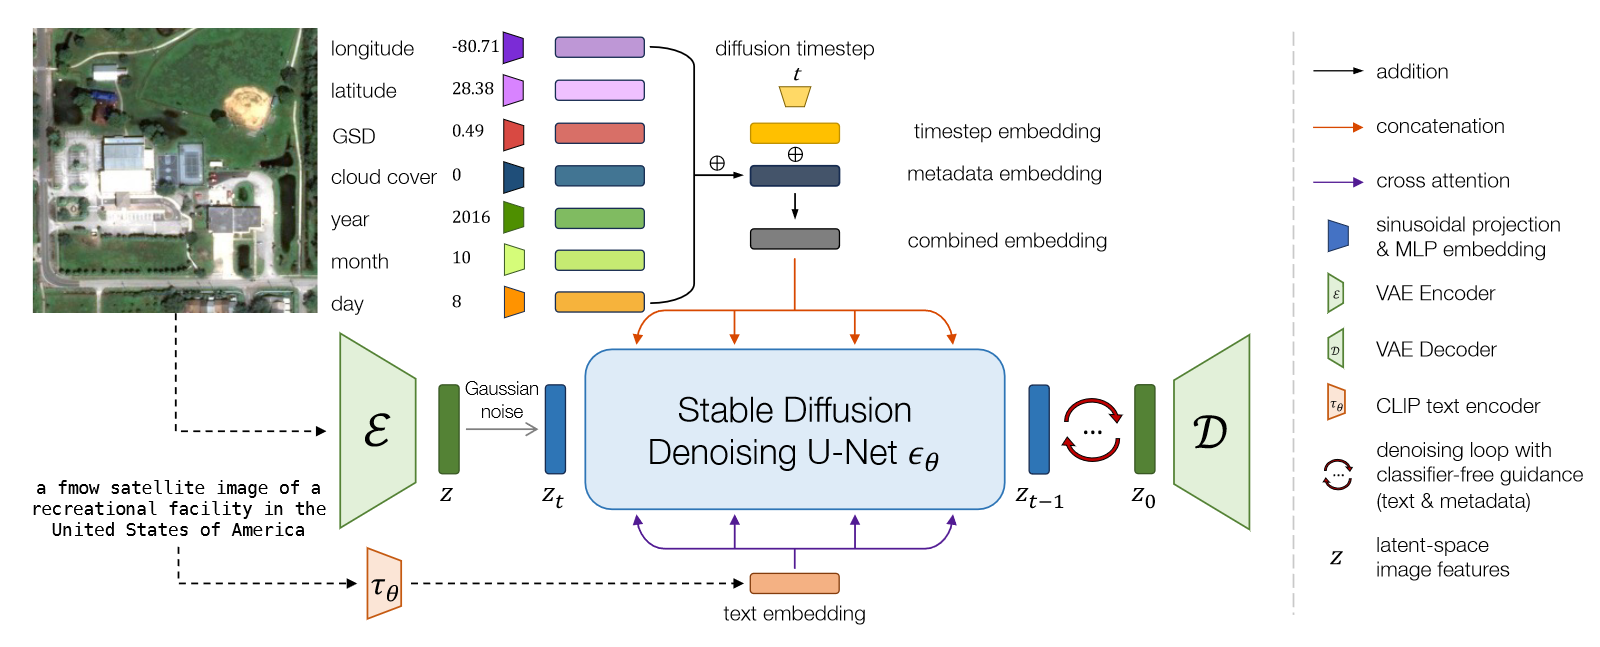
\includegraphics[width=\linewidth]{diffusionsat_base.png}
          \caption{\scriptsize High-level sampling distribution for the DiffusionSat base model.}
        \end{figure}
      \end{column}
    \end{columns}
    \bottomleftrefs
  \end{frame}
\end{refsection}

  

  \begin{refsection}
    \begin{frame}{DiffusionSat+3DControlNet: Framework Overview}
      \begin{figure}
        \centering
        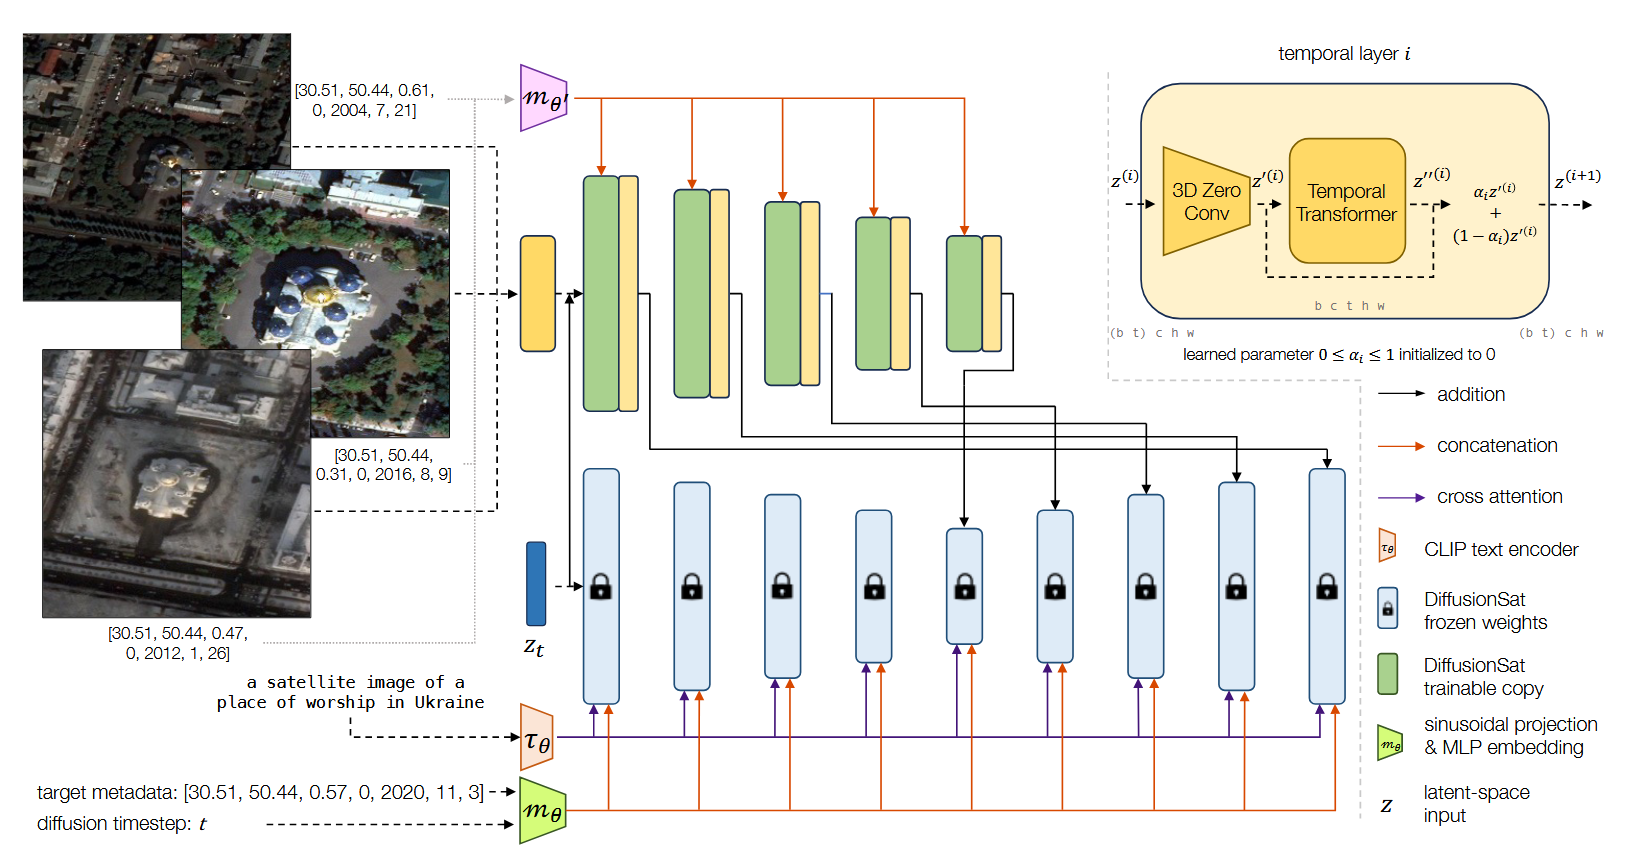
\includegraphics[width=0.9\linewidth]{diffusionsat.png}
        \caption[]{\scriptsize 3DControlNet in DiffusionSat~\parencite{diffusionset2024}.}
      \end{figure}
      \bottomleftrefs
    \end{frame}
    \end{refsection}

  \begin{refsection}
  \begin{frame}{DiffusionSat+3DControlNet: Temporal Prediction Results}
    \begin{figure}
      \centering
      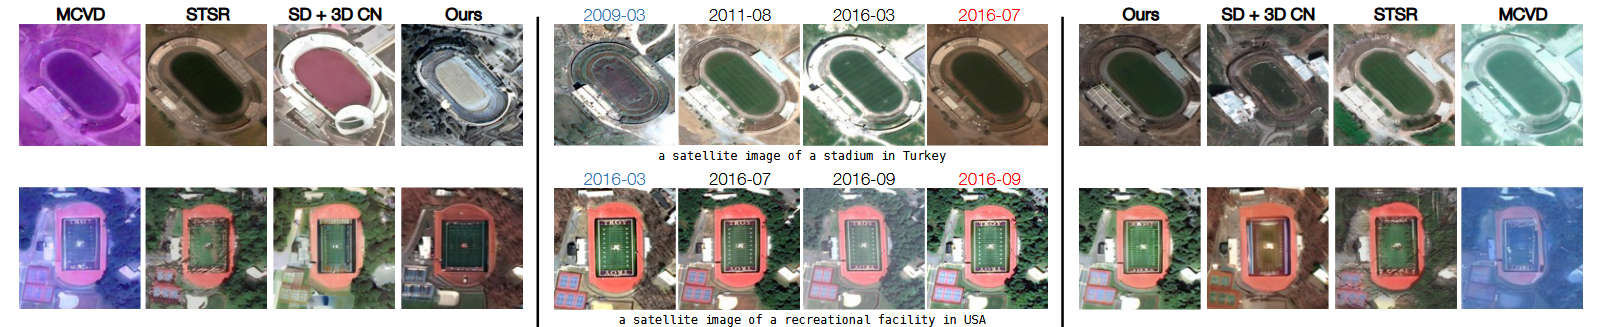
\includegraphics[width=1.0\linewidth]{diffusionsat_temporal_results.png}
      \caption[]{\scriptsize Generated samples from the fMoW-temporal, for temporal prediction~\parencite{diffusionset2024}.}
    \end{figure}
    \begin{table}[h]
      \centering
      \scriptsize
      \begin{tabular}{l|ccc|ccc}
        \toprule
        \multirow{2}{*}{Model} & \multicolumn{3}{c|}{$t' > t$} & \multicolumn{3}{c}{$t' < t$} \\
        & SSIM$\uparrow$ & PSNR$\uparrow$ & LPIPS$\downarrow$ & SSIM$\uparrow$ & PSNR$\uparrow$ & LPIPS$\downarrow$ \\
        \midrule
        SD + 3D CN & 0.2027 & 11.0536 & 0.5523 & 0.2181 & 11.3004 & 0.5342 \\
        DiffusionSat + CN & 0.3297 & 13.6938 & 0.5062 & 0.2862 & 12.4990 & 0.5307 \\
        \textbf{DiffusionSat + 3D CN} & \textbf{0.3983} & \textbf{13.7886} & \textbf{0.4304} & \textbf{0.4293} & \textbf{14.8699} & \textbf{0.3937} \\
        \bottomrule
      \end{tabular}
      \caption[]{\scriptsize Table 4: Sample quality quantitative results on fMoW-temporal validation data. $t' > t$ represents generating an image in the past given a future image, and $t' < t$ is the task for generating a future image given a past image.}
    \end{table}
    \bottomleftrefs
  \end{frame}
  \end{refsection}

    
  \begin{refsection}
  \begin{frame}{DiffusionSat+3DControlNet:Super-Resolution Results}
    \begin{figure}
      \centering
      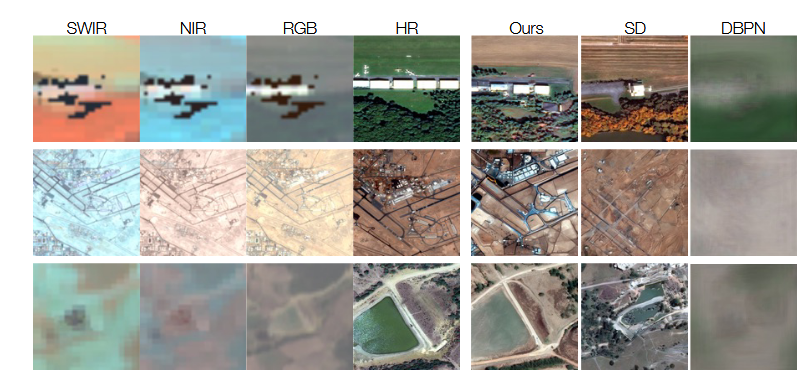
\includegraphics[width=0.9\linewidth]{diffusionsat_sr_results.png}
      \caption[]{\scriptsize Example results: DiffusionSat for multi-spectral super-resolution~\parencite{diffusionset2024}.}
    \end{figure}
    \bottomleftrefs
  \end{frame}
  \end{refsection}


\begin{refsection}
  \begin{frame}
    \centering
    \vspace{2.5cm}
    {\LARGE \textbf{Further Discussion}}
  \end{frame}
\end{refsection}

 
%--- Generative Models for Data Augmentation ---
\begin{refsection}
  \begin{frame}{Using Gen AI to Make New Images}
    \begin{itemize}
      \item Generative models can create new, realistic images.
      \item We can use them to make more training data.
      \item Example: Give a “before” image and a description, get a new “after” image.
    \end{itemize}
    \centering
    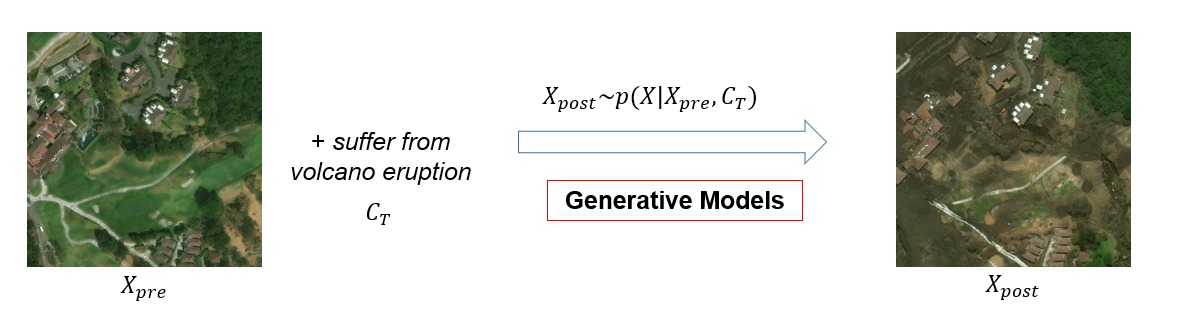
\includegraphics[width=1.0\linewidth]{diffusion_editing.png}
  \end{frame}
  \end{refsection}

  
\begin{refsection}
  \begin{frame}
    \centering
    \vspace{2.5cm}
    {\LARGE \textbf{Supplymentary}}
  \end{frame}
\end{refsection}

\begin{refsection}
  \begin{frame}{How Do We Augment Data?}
    \textbf{Classic Methods:}
      \begin{itemize}
        \item Flip, rotate, crop, change colors, etc.
      \end{itemize}
      \textbf{Modern Methods:}
      \begin{itemize}
        \item Mix two images together (Mixup)~\parencite{zhangMixupEMPIRICALRISK2018}.
        \item Cut and paste parts of images (CutMix)~\parencite{yunCutMixRegularizationStrategy2019}.
      \end{itemize}
    \begin{minipage}{0.58\linewidth}
      \begin{figure}
        \centering
        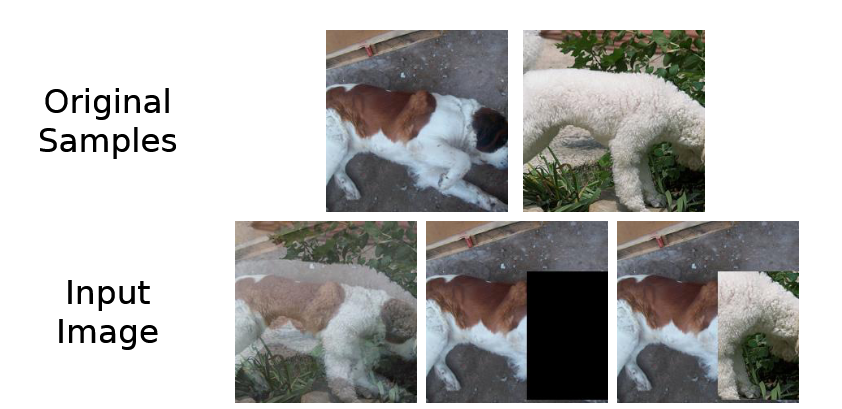
\includegraphics[width=0.6\linewidth]{aug_new_methods.png}
        \caption[]{\scriptsize Illustration of modern augmentation methods. From Left to Right: Mixup~\parencite{zhangMixupEMPIRICALRISK2018}, Cutout~\parencite{devriesImprovedRegularizationConvolutional2017}, and CutMix~\parencite{yunCutMixRegularizationStrategy2019}.}
      \end{figure}
    \end{minipage}
    \hfill
    \begin{minipage}{0.4\linewidth}
      \textbf{Soft Label Example (CutMix):}
      % \vspace{0.5em}
      \tiny
      \begin{equation*}
        \text{cutmix\_label} = \lambda \cdot \text{label}_A + (1 - \lambda) \cdot \text{label}_B
      \end{equation*}
      \vspace{-0.5em}
      \begin{equation*}
        \text{Example:} \quad \lambda = 0.5, \quad \text{label}_A = [1, 0], \quad \text{label}_B = [0, 1]
      \end{equation*}
      \vspace{-0.5em}
      \begin{equation*}
        \text{cutmix\_label} = 0.5 \times [1, 0] + 0.5 \times [0, 1] = [0.5, 0.5]
      \end{equation*}
     
  
    \end{minipage}
    \bottomleftrefs
  \end{frame}
  \end{refsection}
  
  
\begin{refsection}
\begin{frame}{Generative Models for Data Augmentation}
  \begin{minipage}{0.7\linewidth}
    % \centering
    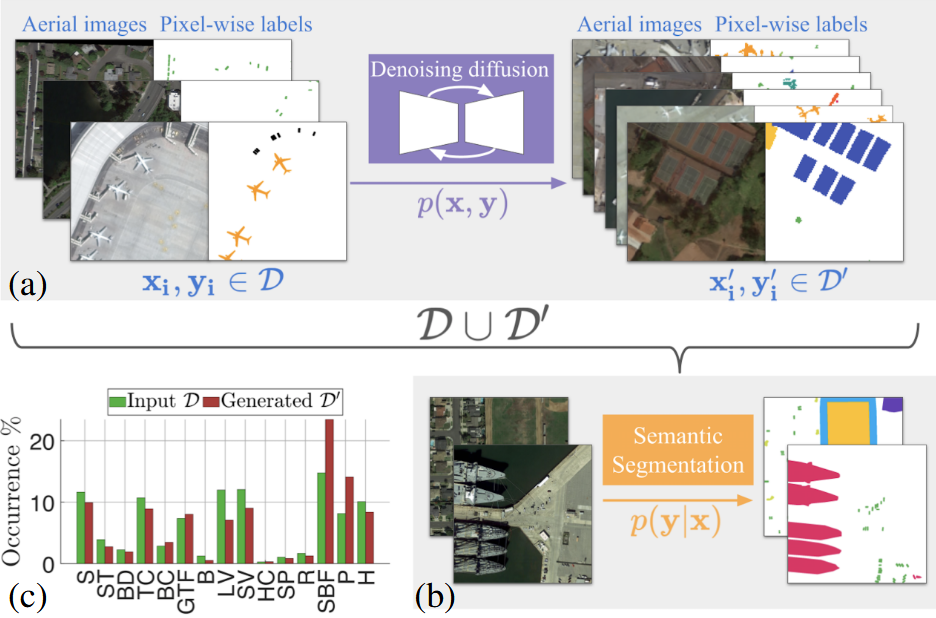
\includegraphics[width=0.9\linewidth]{satsyn.png}
  \end{minipage}%
  \hfill
  \begin{minipage}{0.3\linewidth}
    \scriptsize
    SatSyn~\parencite{tokerSatSynthAugmentingImageMask2024} proposes a generative model (diffusion model) to generate both images and corresponding masks for satellite segmentation. The synthetic dataset is used for data augmentation, yielding significant quantitative improvements in satellite semantic segmentation compared to other data augmentation methods.
  \end{minipage}
  \bottomleftrefs
\end{frame}
\end{refsection}

\begin{refsection}
\begin{frame}{Application in Remote Sensing Image Generation: Text2Earth}
  \begin{figure}
    \centering
    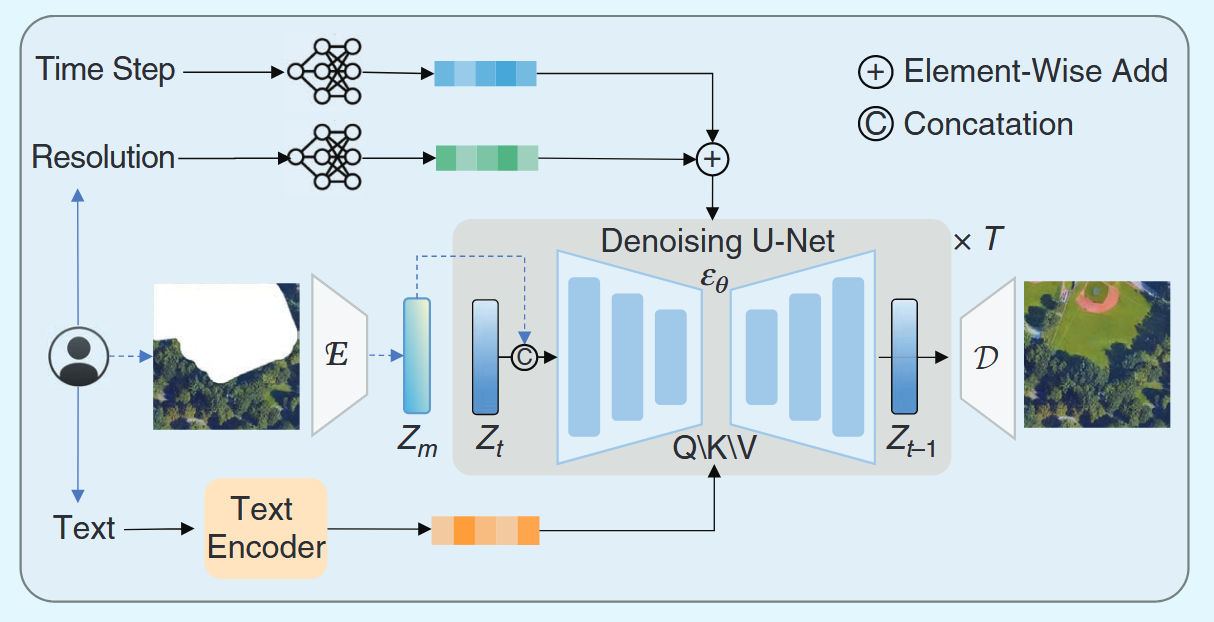
\includegraphics[width=0.9\linewidth]{text2earth.png}
    \caption[]{\scriptsize Text2Earth: Foundation model for text-driven Earth observation~\parencite{text2earth2025}.}
  \end{figure}
  \bottomleftrefs
\end{frame}
\end{refsection}

\begin{refsection}
\begin{frame}{Text2Earth: Example Results}
  \begin{figure}
    \centering
    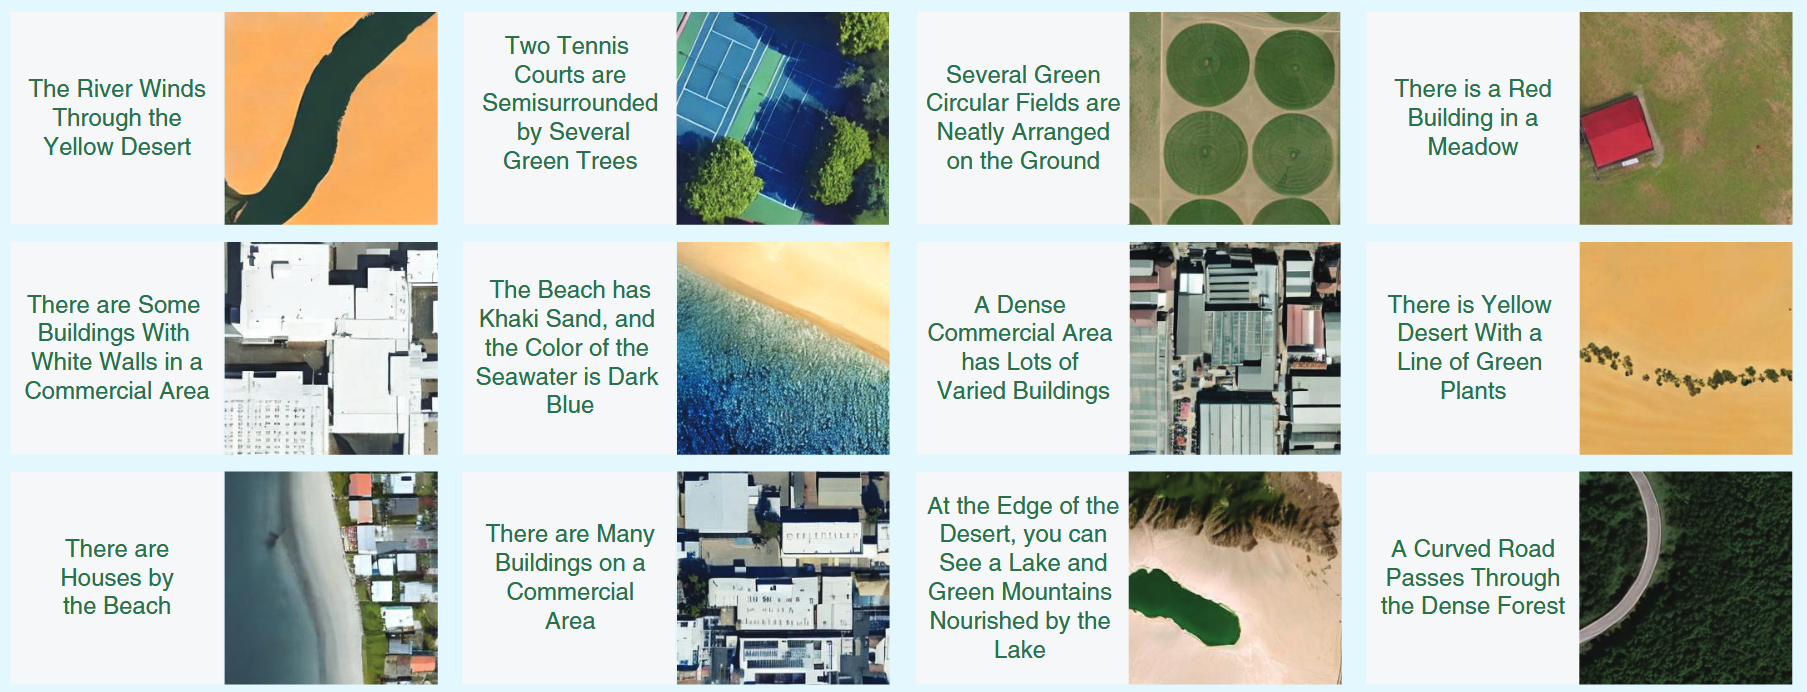
\includegraphics[width=0.9\linewidth]{text2earth_results.png}
    \caption[]{\scriptsize Example results generated by Text2Earth~\parencite{text2earth2025}.}
  \end{figure}
  \bottomleftrefs
\end{frame}
\end{refsection}

\begin{refsection}
\begin{frame}{Application in Remote Sensing Image Generation: CRS-Diff}
\begin{figure}
  \centering
  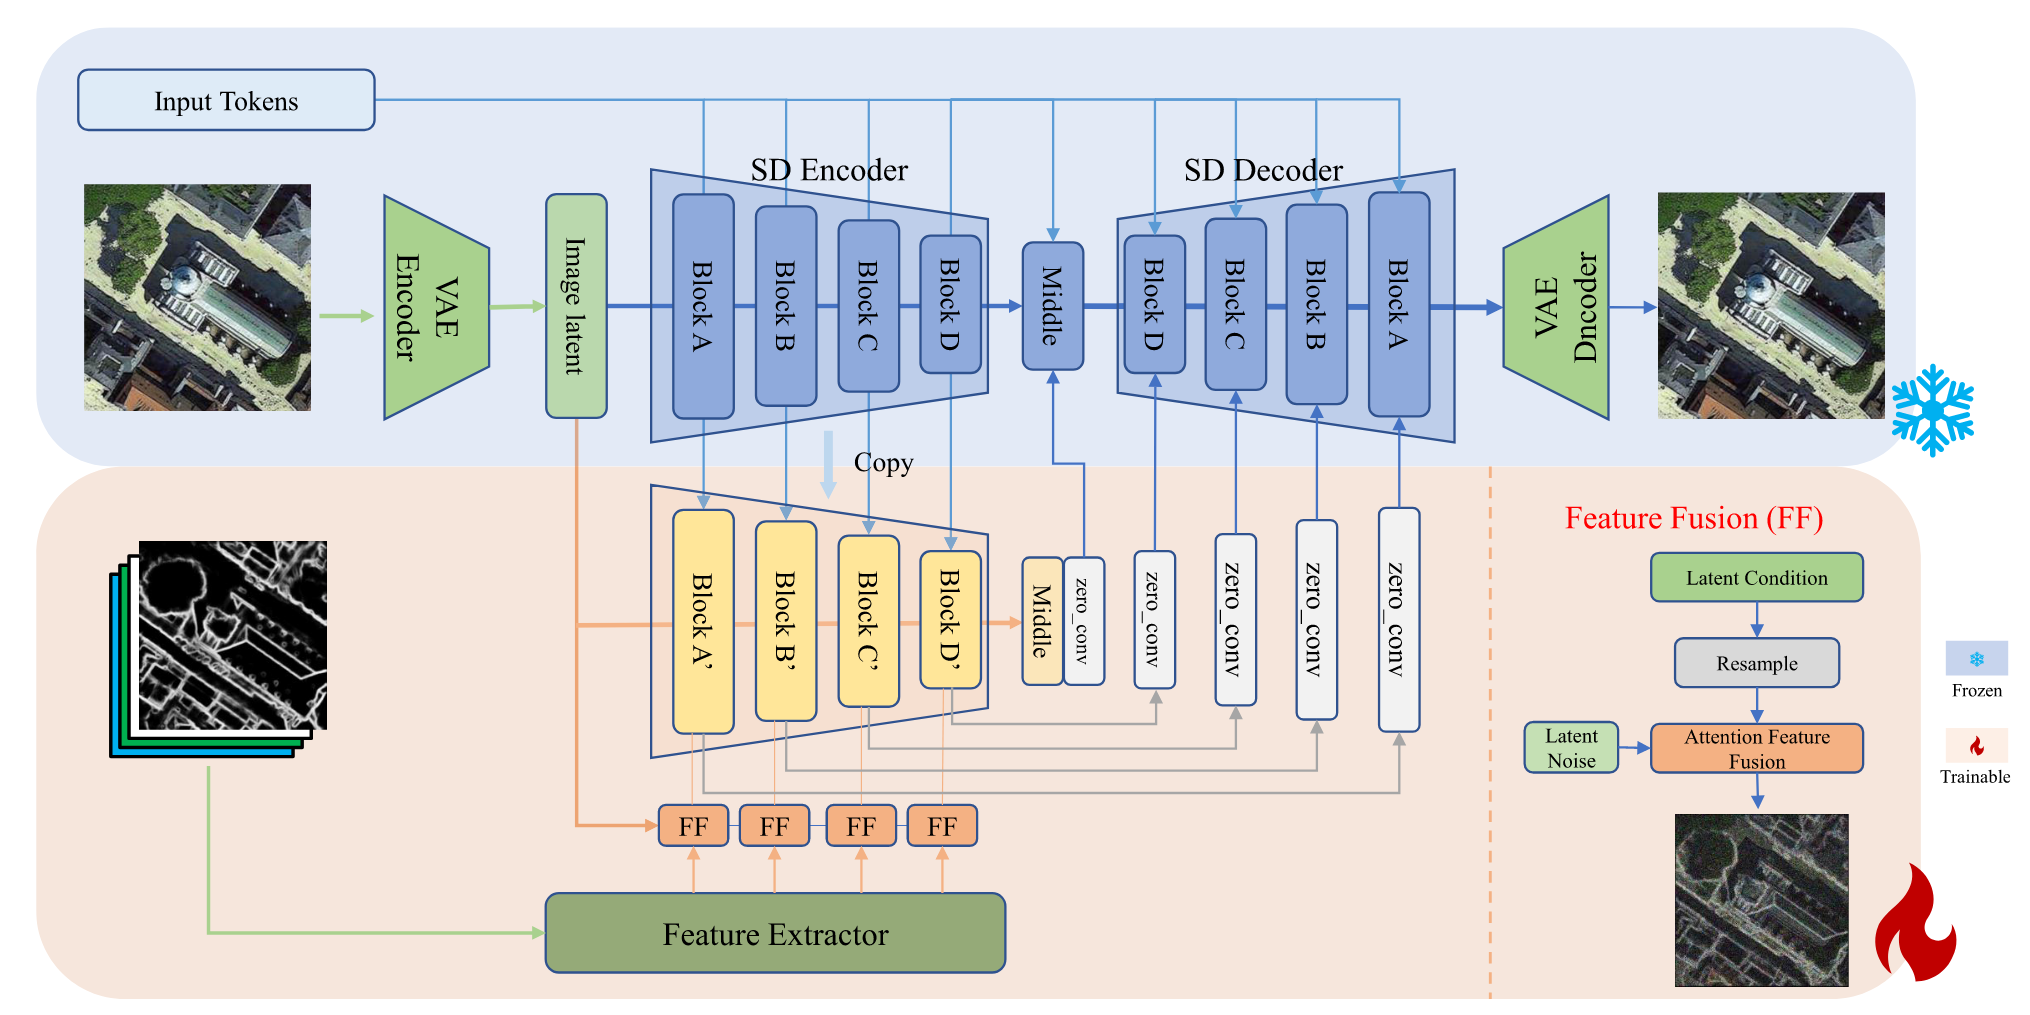
\includegraphics[width=0.9\linewidth]{crsdiff.png}
  \caption[]{\scriptsize CRS-Diff: Controllable remote sensing image generation framework~\parencite{tang2024crsdiff}.}
\end{figure}
\bottomleftrefs
\end{frame}
\end{refsection}

\begin{refsection}
\begin{frame}{CRS-Diff: Example Results}
\begin{figure}
  \centering
  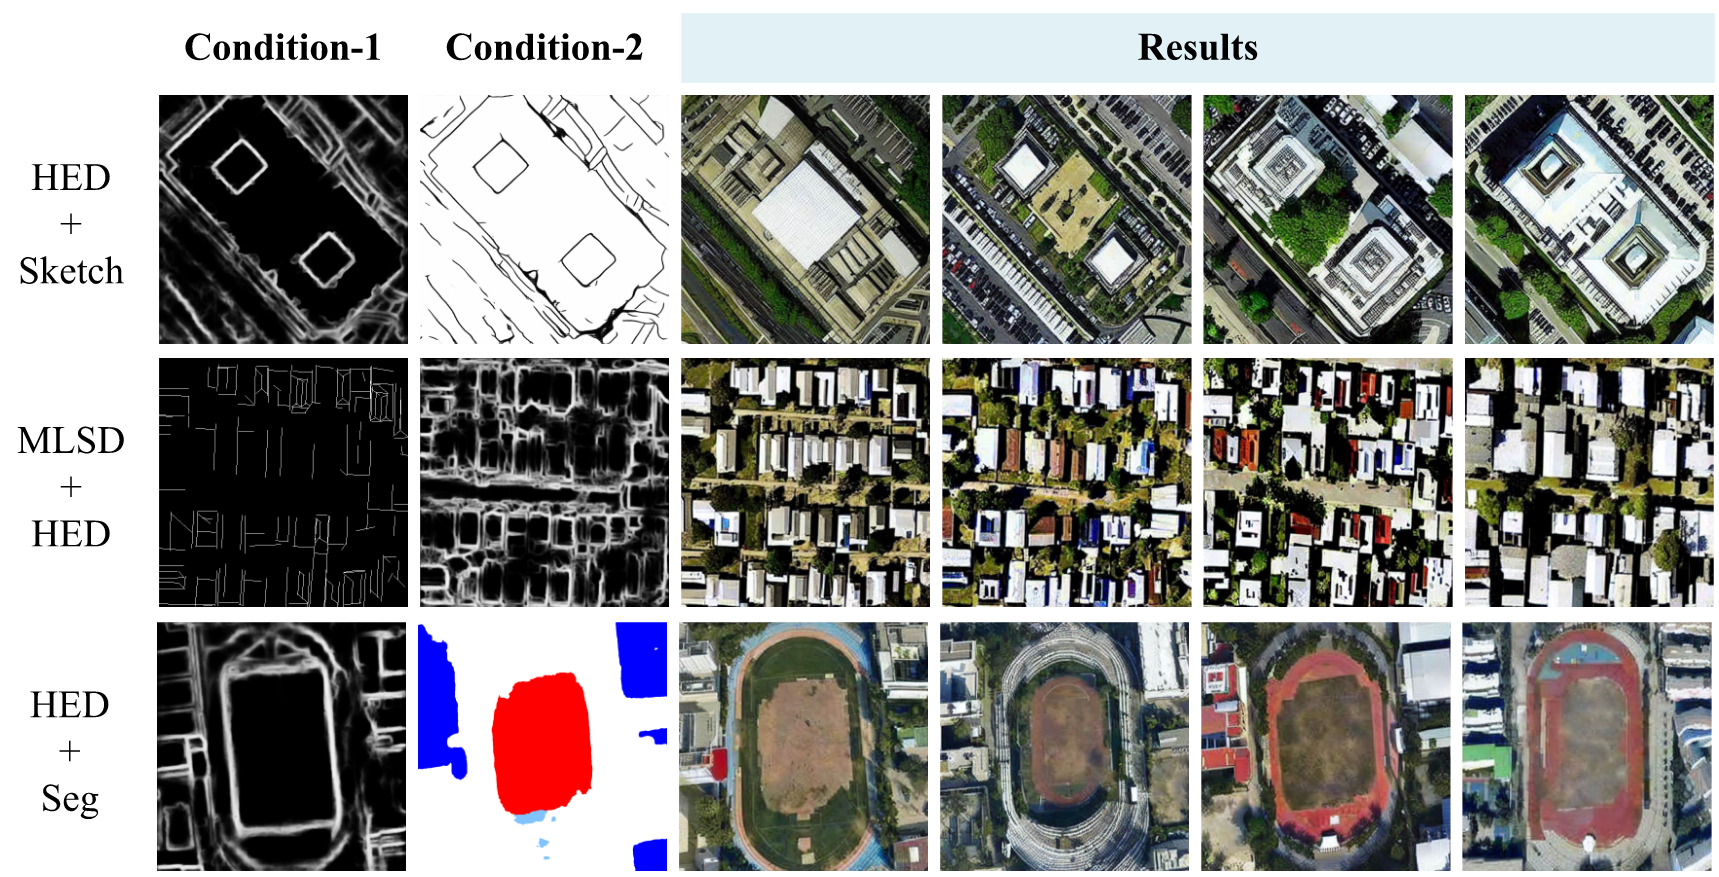
\includegraphics[width=0.9\linewidth]{crsdiff_results.png}
  \caption[]{\scriptsize Example results generated by CRS-Diff~\parencite{tang2024crsdiff}.}
\end{figure}
\bottomleftrefs
\end{frame}
\end{refsection}